\chapter{Xây dựng ứng dụng\\tìm kiếm đối tượng trên ảnh}
\label{chapter:application}
\ifpdf
    \graphicspath{{Chapter5/Chapter5Figs/PNG/}{Chapter5/Chapter5Figs/PDF/}{Chapter5/Chapter5Figs/}}
\else
    \graphicspath{{Chapter5/Chapter5Figs/EPS/}{Chapter5/Chapter5Figs/}}
\fi
\markboth{\MakeUppercase{\thechapter. Xây dựng ứng dụng tìm kiếm đối tượng trên ảnh}}{\thechapter. Xây dựng ứng dụng tìm kiếm đối tượng trên ảnh}

Trên cơ sở các phương pháp đã nghiên cứu và những kết quả thực nghiệm của phương pháp đề xuất, chúng tôi tiến hành xây dựng ứng dụng tìm kiếm đối tượng trên ảnh nhằm thực nghiệm phương pháp đề xuất trên môi trường thực tế và tăng tính ứng dụng cho đề tài.

Trong chương này, trước tiên chúng tôi sẽ giới thiệu tổng quan về mục đích và các chức năng chính của ứng dụng (mục \ref{c5-tongquan}). Sau đó là bước thiết kế kiến trúc, tổ chức các thành phần và giao diện của ứng dụng (mục \ref{c5-thietke}). Cuối cùng là bước cài đặt, thử nghiệm và đánh giá kết quả của hệ thống đã cài đặt (mục \ref{c5-caidat}).

\section{Tổng quan ứng dụng}
\label{c5-tongquan}

	\subsection{Mục đích và phạm vi của ứng dụng}
Như đã giới thiệu trong mục ..., các hệ thống truy vấn ảnh có vô vàn ứng dụng khác nhau trong thực tế. Trong đề tài này, chúng tôi xây dựng ứng dụng nhằm phục vụ mục đích cơ bản là tìm kiếm đối tượng trên những kho dữ liệu ảnh với kích thước có thể lên tới hàng trăm ngàn ảnh. Đó có thể là kho dữ liệu ảnh của một tổ chức, công ty về một lĩnh vực nào đó. Hay xa hơn, ứng dụng này có thể phát triển cho việc tìm kiếm đối tượng trên kho dữ liệu video vì ta hoàn toàn có thể rút trích được hình ảnh từ các frame của video.
	
	\subsection{Các chức năng chính}
Trong ứng dụng này, để tăng tính tiện dụng và gần gũi với người dùng, phía client được xây dựng trên nền tảng thiết bị động. Ứng dụng bao gồm các chức năng chính sau:

-- Chụp hình đối tượng: người dùng có thể sử dụng camera của điện thoại để chụp hình đối tượng và tìm kiếm.

-- Chọn ảnh được lưu trữ trước trong máy: người dùng có thể chọn một ảnh có chứa đối tượng được lưu trữ trong điện thoại, thẻ nhớ để tìm kiếm.

-- Chọn vùng đối tượng: từ ảnh chụp được hay ảnh được lưu trữ sẵn trong máy, để nâng cao độ chính xác của việc tìm kiếm, người dùng có thể khoanh vùng đối tượng cần tìm trên ảnh.

\section{Thiết kế ứng dụng}
\label{c5-thietke}

	\subsection{Kiến trúc}
Kiến trúc của chương trình được chia làm 3 thành phần chính:

-- Client side: là một ứng dụng di động chạy trên hệ điều hành Android cho phép người dùng chụp ảnh hoặc chọn ảnh từ file, sau đó nén và mã hóa và gửi lên web service.

-- Web service: nhận các request từ phía client. Thực hiện điều phối và cân bằng tải để chuyển tiếp các request cho các web server để xử lý. Đồng thời tiếp nhận kết quả xử lý từ các web server để trả về cho từng client tương ứng.

-- Server side: Nhận request từ web service chuyển tiếp lên, xử lý và trả về kết quả cho web service. Việc xử lý ở phía server tốn rất nhiều tài nguyên thế nên nếu lượng request lớn, sẽ rất dễ rơi vào trường hợp thắt cổ chai. Do đó, để tăng sức mạnh cho hệ thống, ứng dụng có thể scale ra nhiều server để chia tải.

Hình \ref{FigArchitecture} minh họa cho mô hình hoạt động tổng quan của hệ thống.

\begin{figure}[!htbp]
  \begin{center}
    \leavevmode
    \ifpdf
      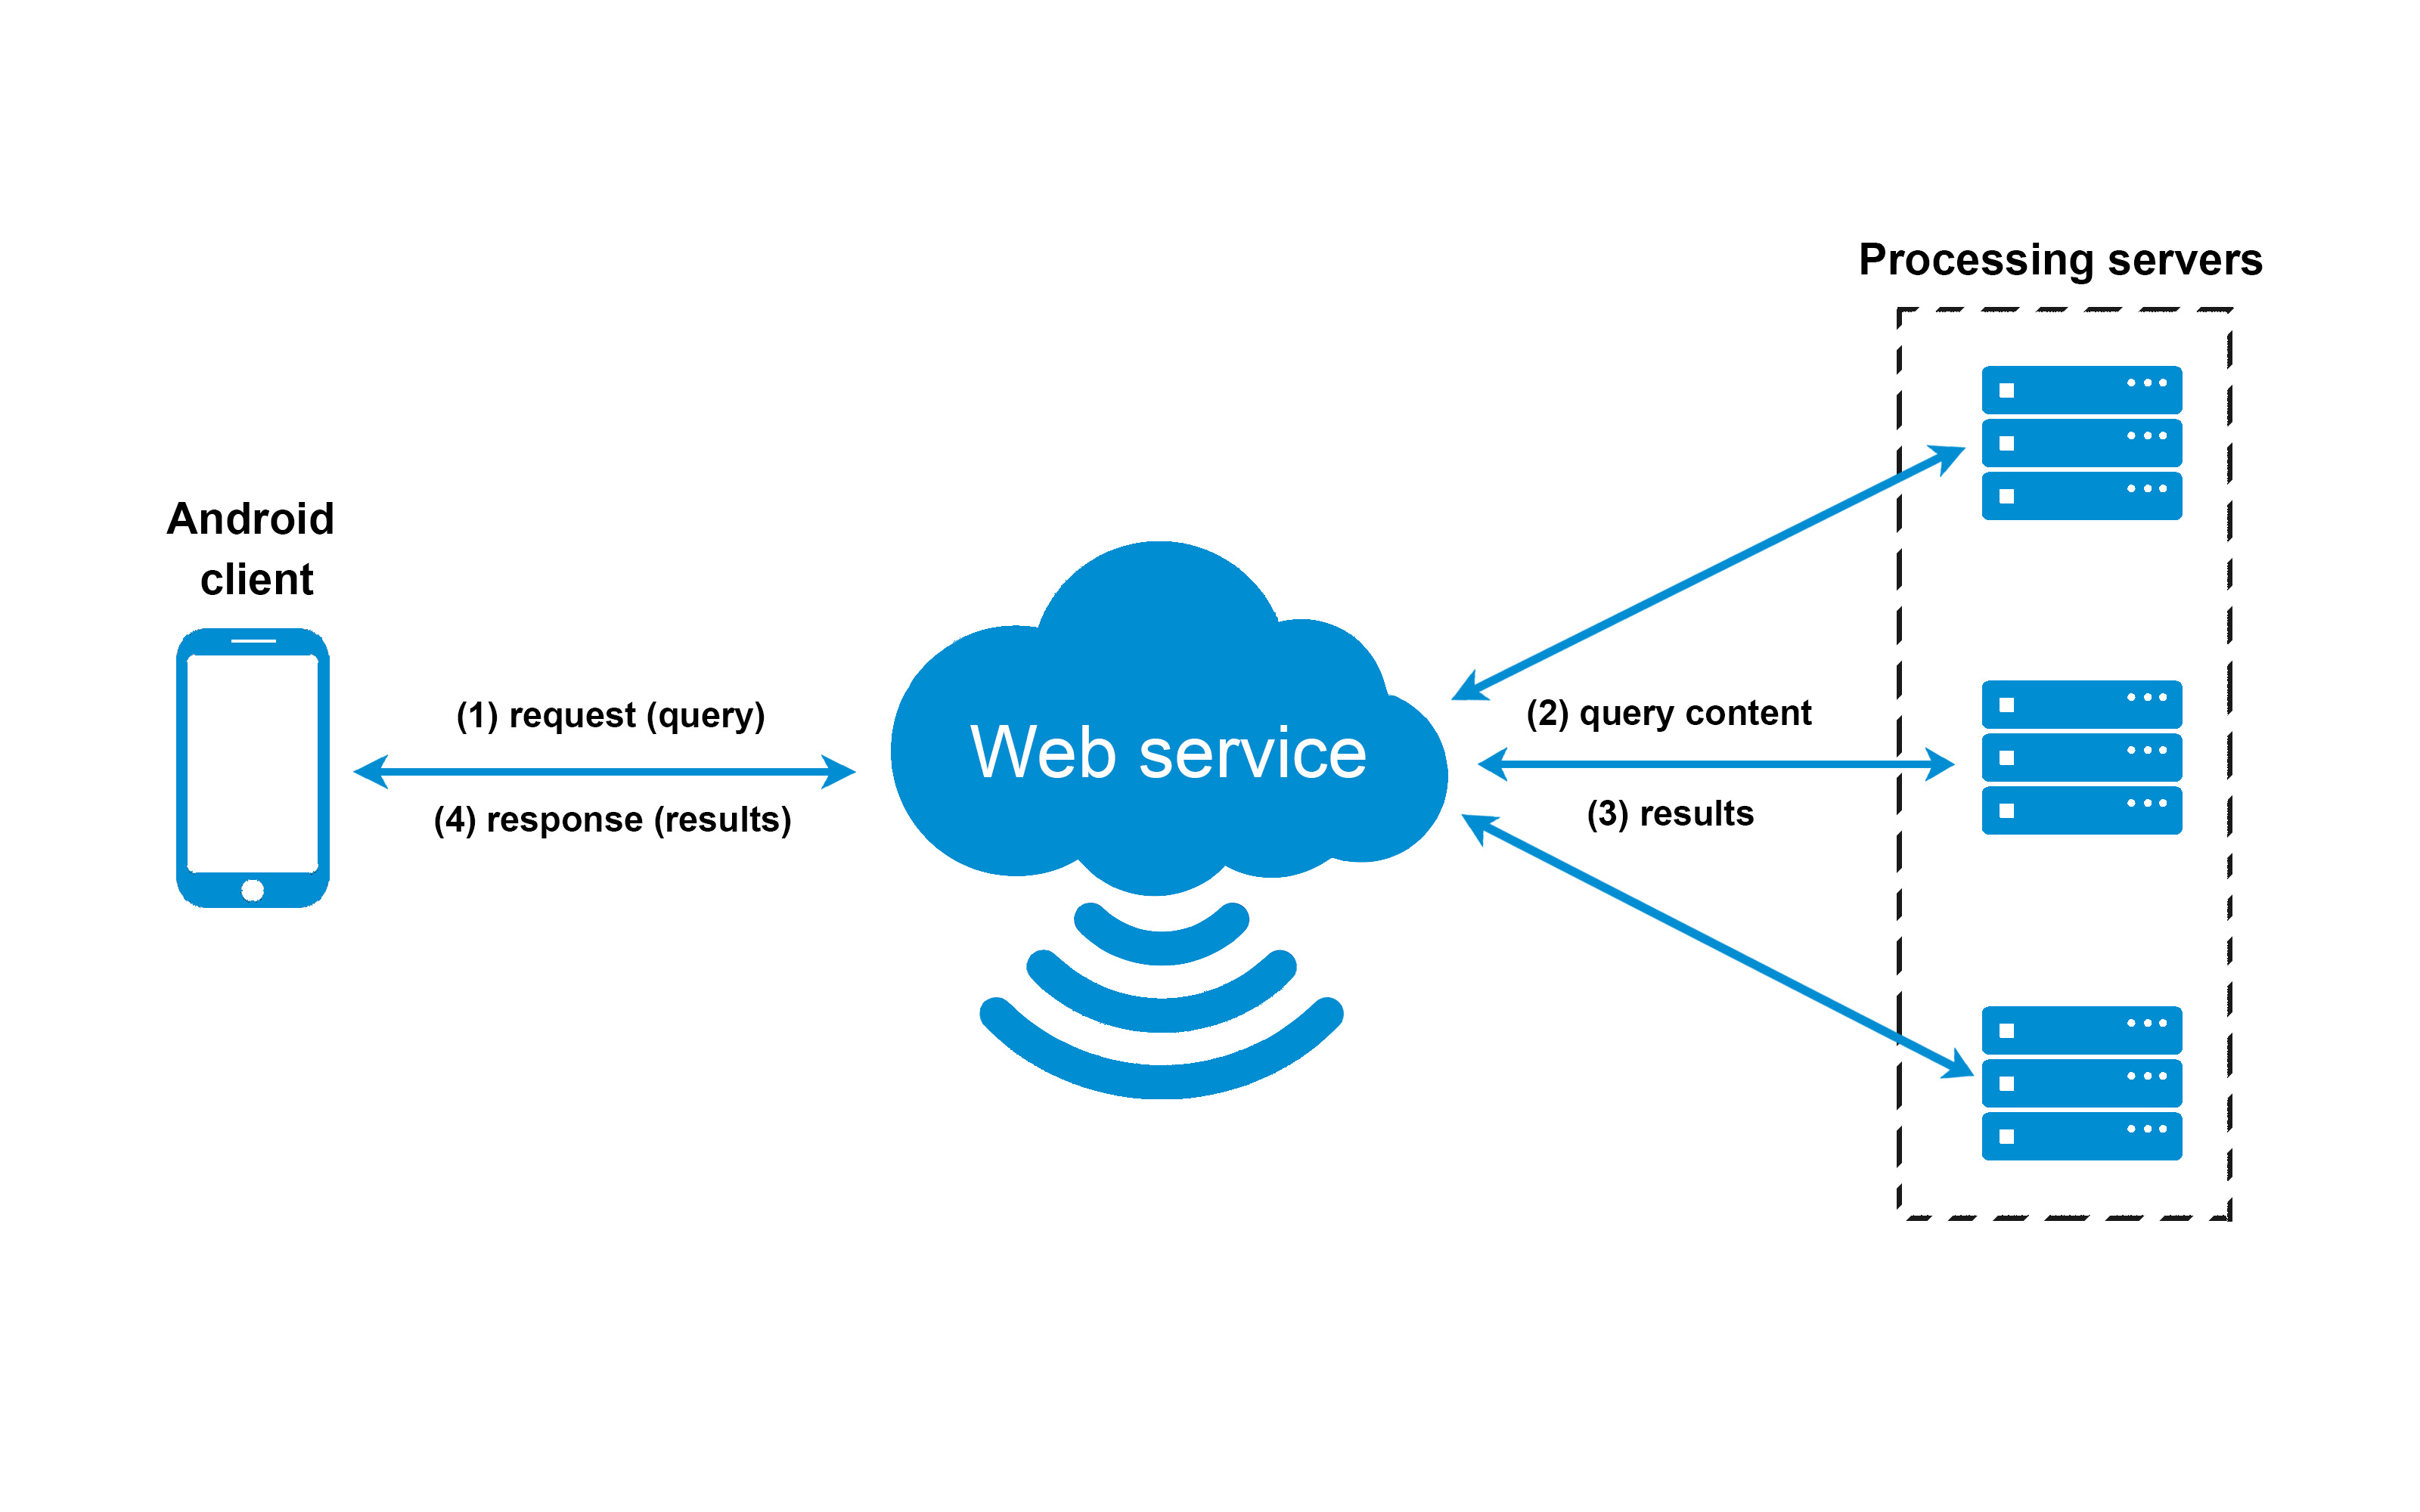
\includegraphics[scale=0.14]{architecture}
    \else
      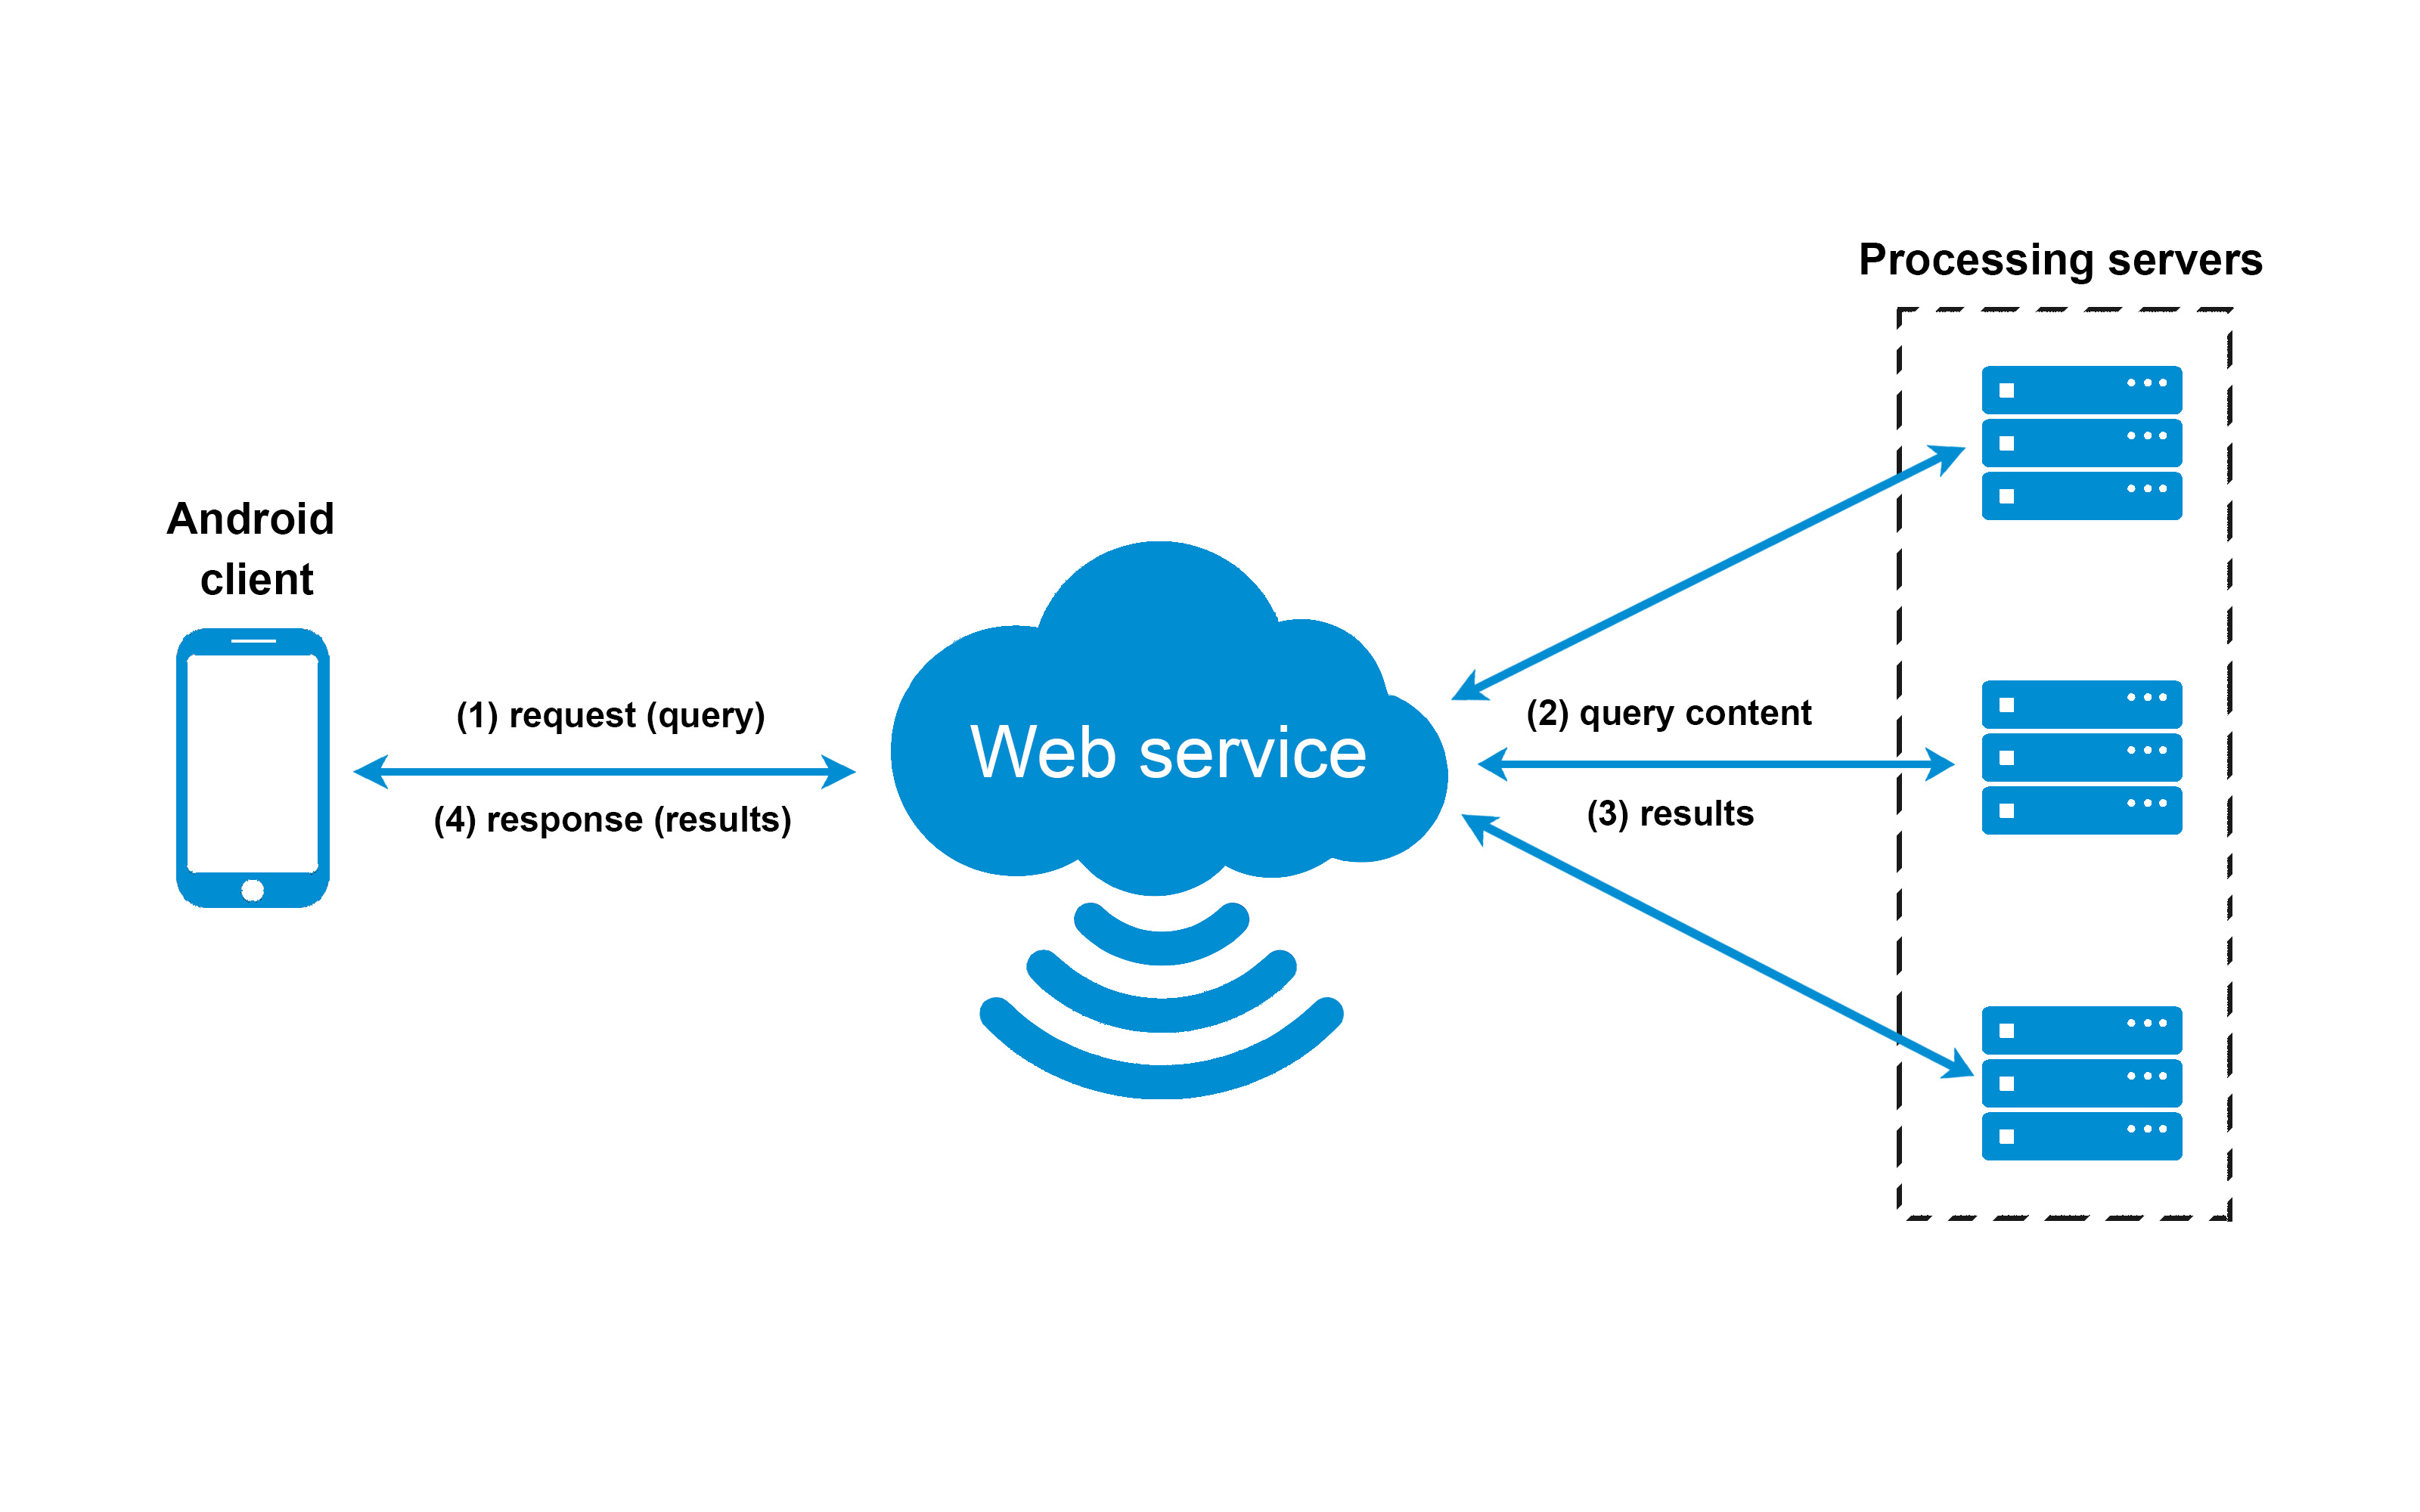
\includegraphics[scale=0.14]{architecture}
    \fi
    \caption[Kiến trúc tổng quan của hệ thống]{Kiến trúc tổng quan của hệ thống.}
    \label{FigArchitecture}
  \end{center}
\end{figure}

\subsubsection{Client side}
Ứng dụng client là phần tương tác trực tiếp với người dùng. Nhiệm vụ của client là cung cấp cho người dùng một giao diện để tương tác trong quá trình chọn ảnh để request. Do đó nó cần đáp ứng được các yêu cầu về giao diện thân thiện, tiện dụng và cung cấp đầy đủ các chức năng cho người dùng. Hình \ref{FigAndroidClient} cho thấy kiến trúc tổng quan của client side.

\begin{figure}[!htbp]
  \begin{center}
    \leavevmode
    \ifpdf
      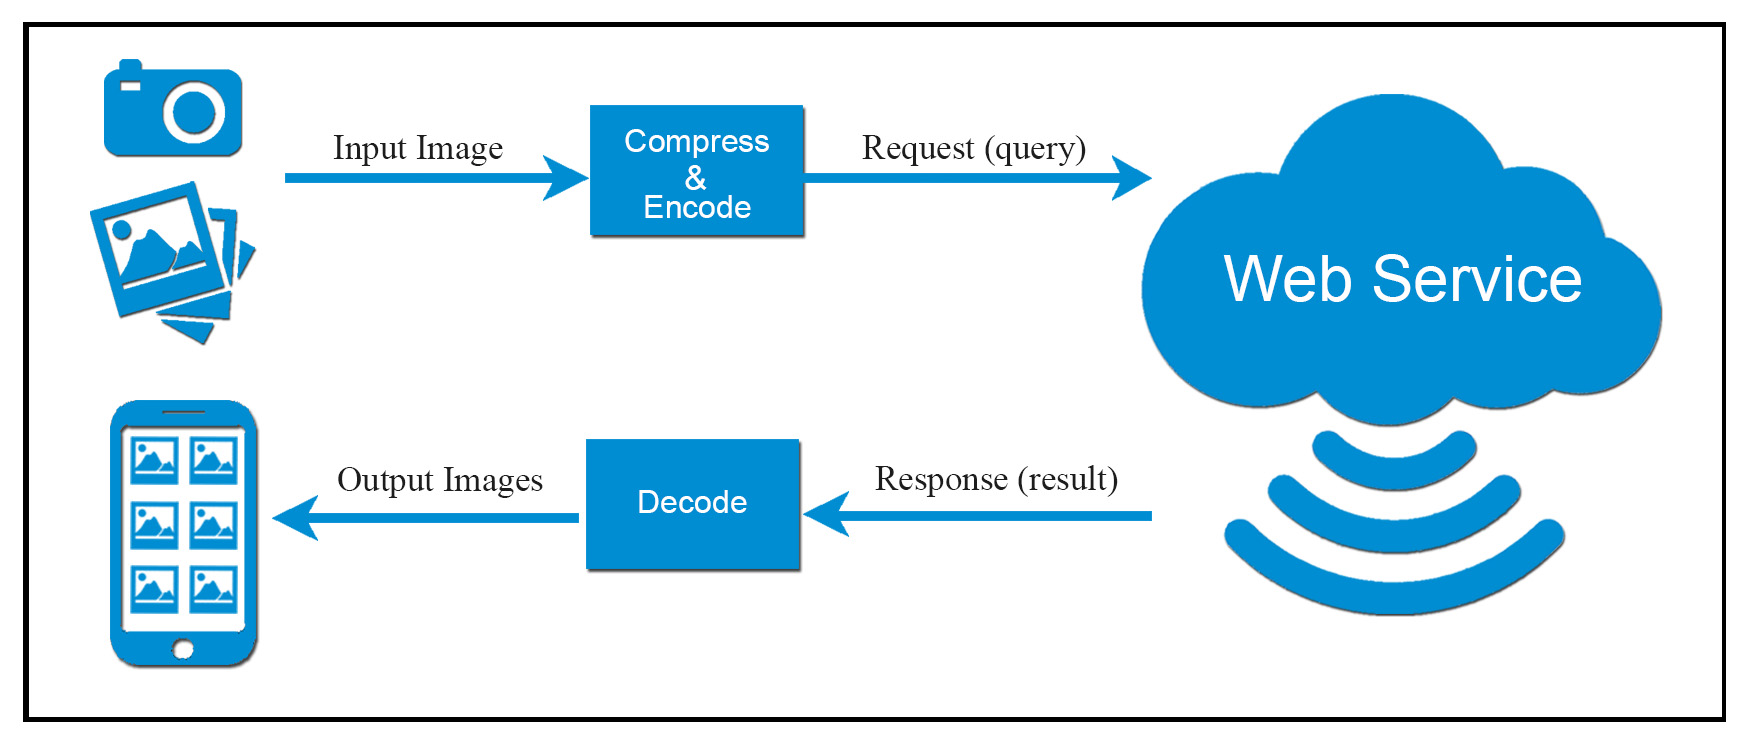
\includegraphics[scale=0.25]{android_client}
    \else
      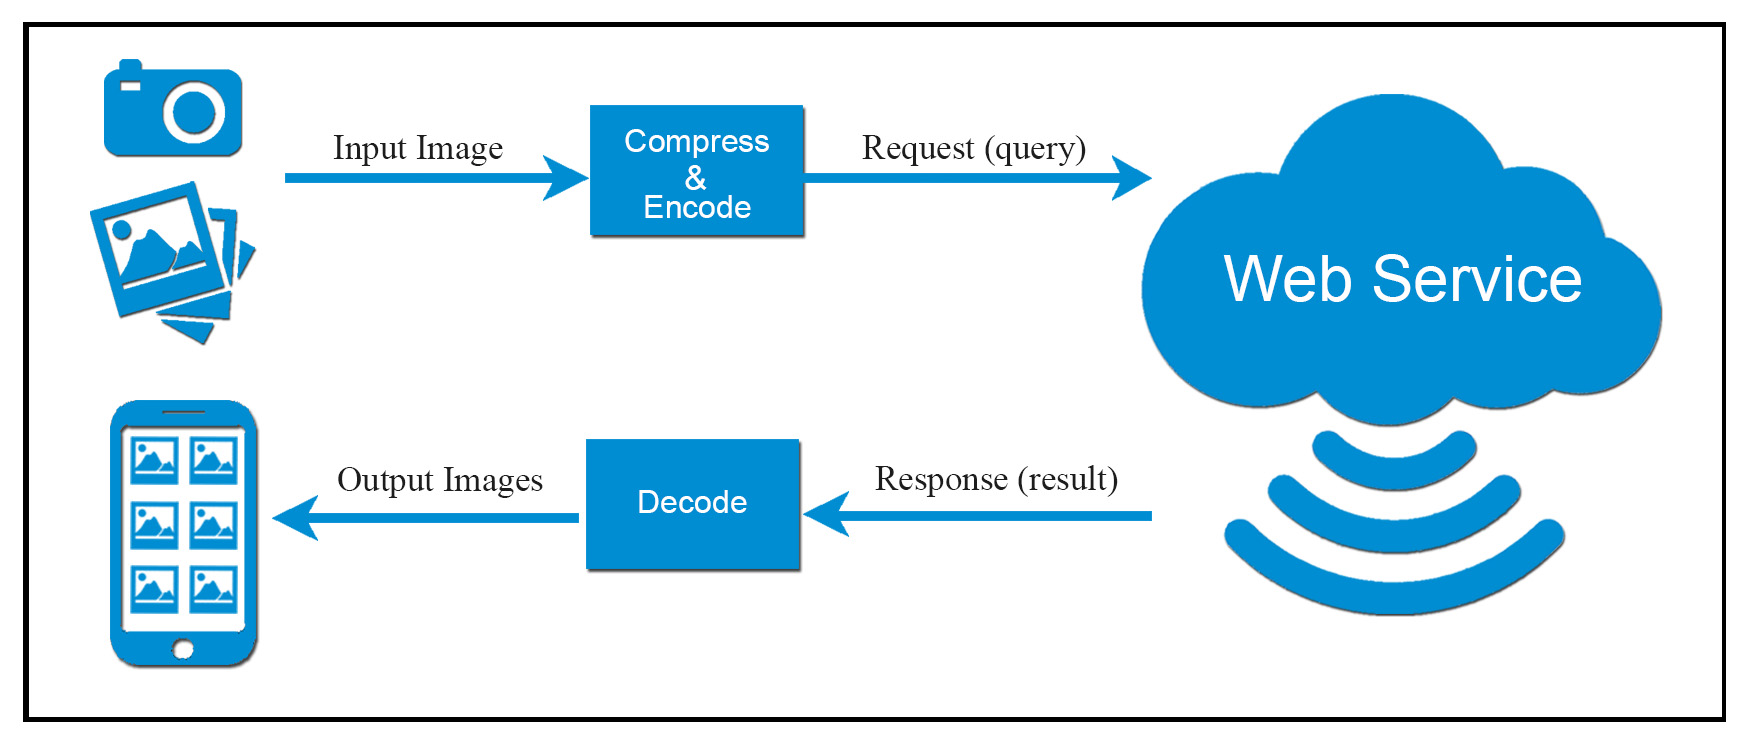
\includegraphics[scale=0.25]{android_client}
    \fi
    \caption[Kiến trúc của client side]{Kiến trúc của client side.}
    \label{FigAndroidClient}
  \end{center}
\end{figure}


Ứng dụng client được xây dựng đơn giản và thân thiện với người dùng. Nó cho phép người dùng được chọn hình ảnh từ camera hoặc hình ảnh được lưu trữ trong bộ nhớ. Để nâng cao độ chính xác, người dùng có thể dùng tay để quét chọn vùng hình ảnh có chứa đối tượng mà mình muốn truy vấn. Sau đó hình ảnh sẽ được gửi cho web service. Và khi có kết quả trả về từ web service, ứng dụng sẽ hiển thị danh sách các hình ảnh trả về dưới dạng các thumbnail. Nếu người dùng muốn xem hình ảnh lớn hơn, chỉ cần chọn hình ảnh và ứng dụng sẽ gửi request lên web service để lấy hình ảnh chất lượng cao về và hiển thị.

Chi tiết tổ chức của các lớp được thể hiện trong Hình \ref{FigClientFramework}.

\begin{figure}[!htbp]
  \begin{center}
    \leavevmode
    \ifpdf
      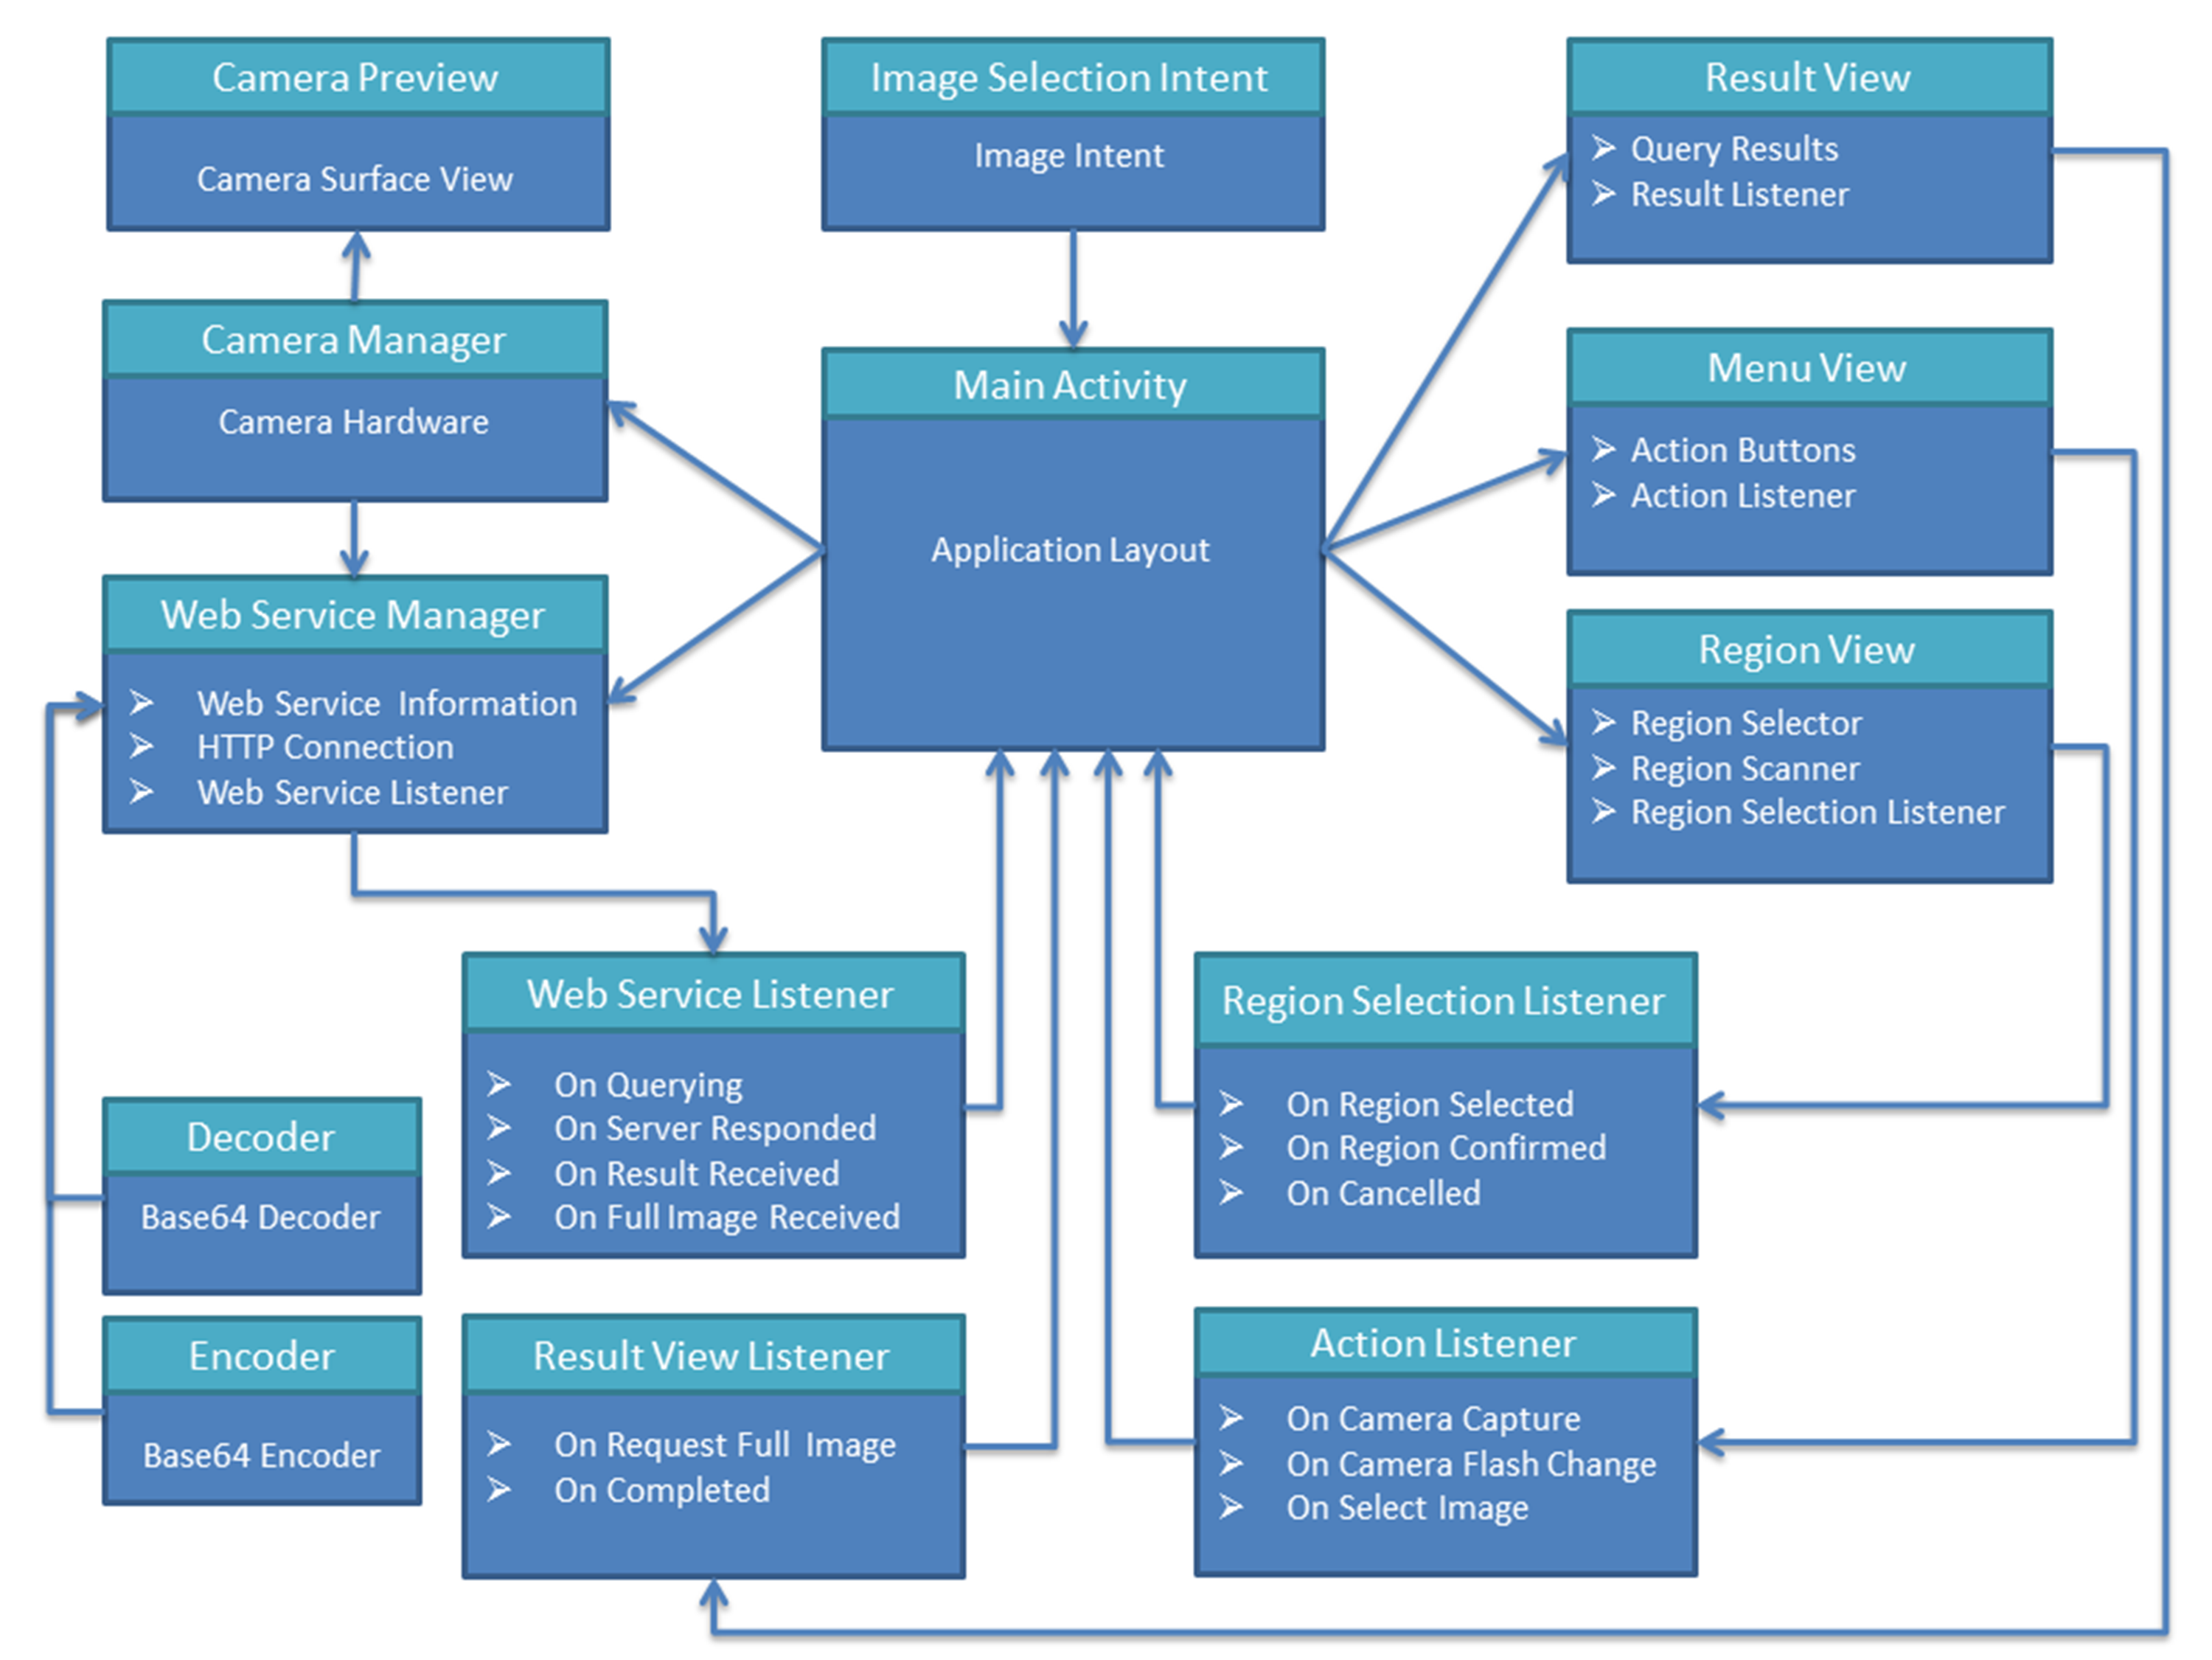
\includegraphics[scale=0.19]{client_framework}
    \else
      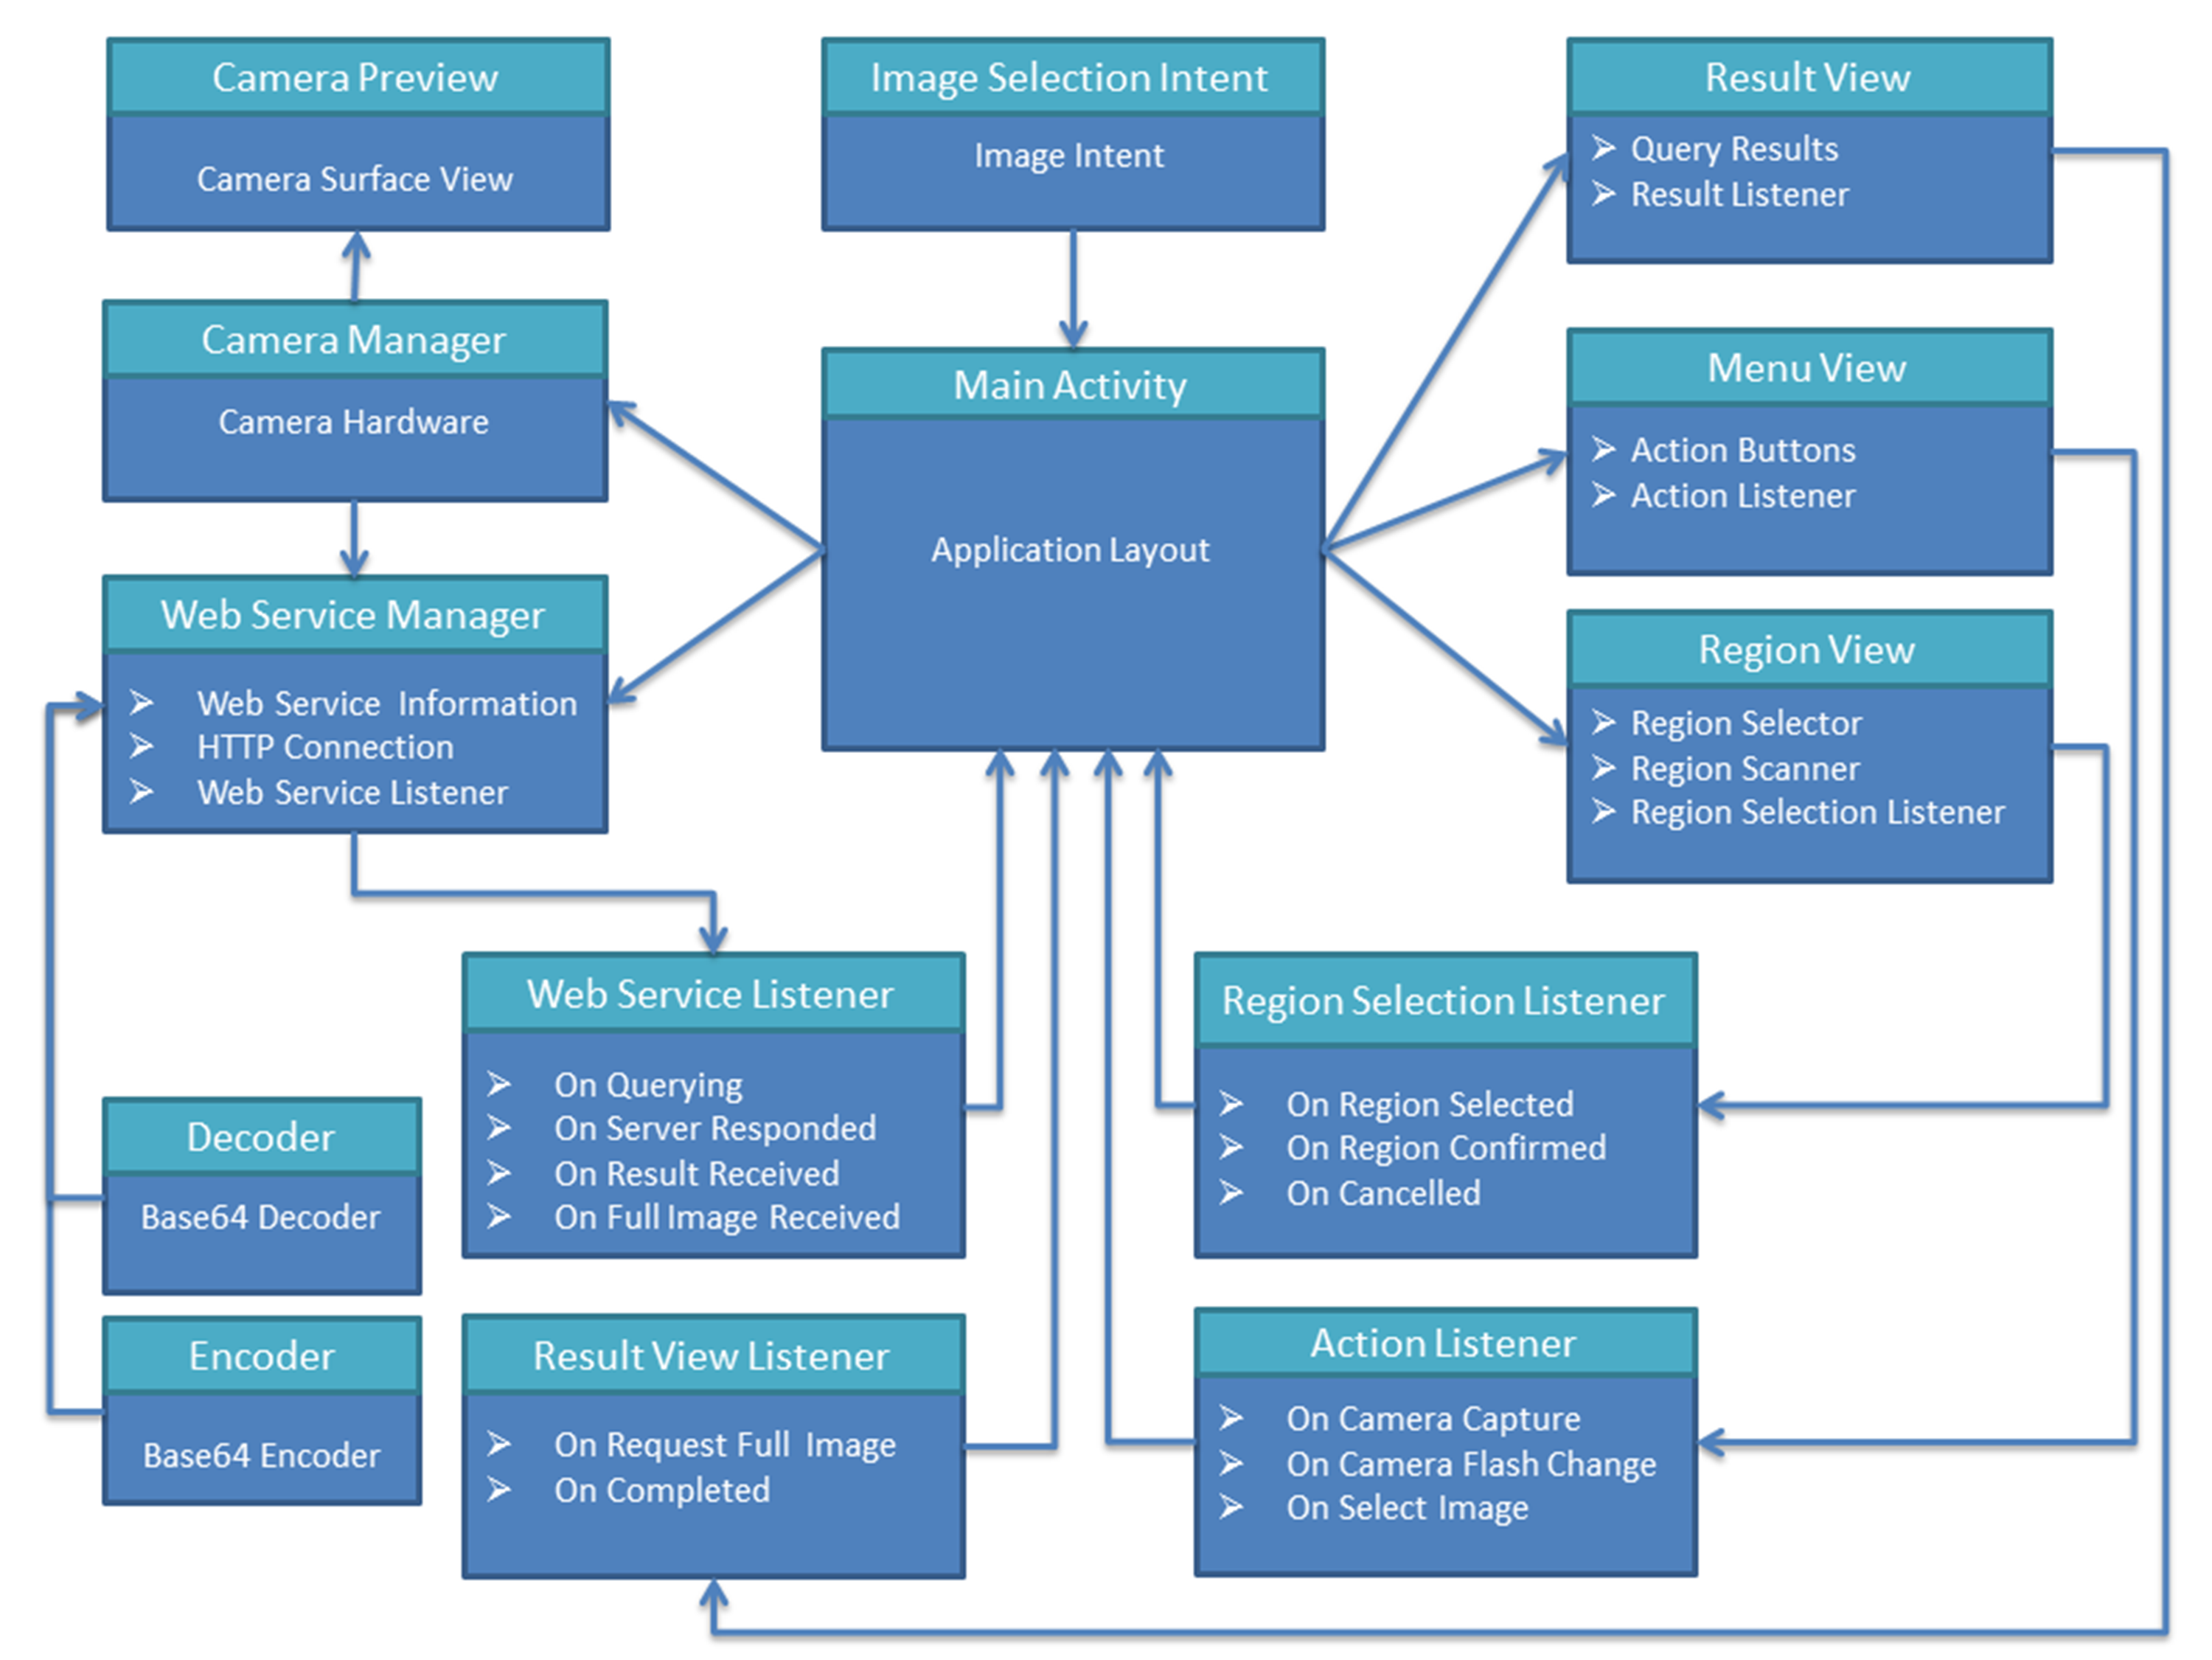
\includegraphics[scale=0.19]{client_framework}
    \fi
    \caption[Sơ đồ tổ chức các lớp của client side]{Sơ đồ tổ chức các lớp của client side.}
    \label{FigClientFramework}
  \end{center}
\end{figure}

\subsubsection{Web service}
Web service đóng vai trò điều phối trung gian giữa client và server. Do đó, web service thực hiện hai nhiệm vụ chính là nhận các request từ các client gửi lên, điều phối để cân bằng tải giữa các server và nhận kết quả trả về từ server để trả lại đúng cho client tương ứng.

Trước tiên, các request do client gửi lên sẽ được đưa vào hàng đợi. Các kết nối của phía server gửi lên cũng được đưa vào một hàng đợi. Controller sẽ làm nhiệm vụ kiểm tra xem liệu có kết nối của server nào đang đợi không để chuyển tiếp request của client đến server đó. Đồng thời, bằng việc sử dụng kỹ thuật long polling, request của client sẽ không được trả về ngay mà sẽ bị giữ lại để chờ đợi kết quả từ phía server. Sau khi xử lý và lấy được kết quả, server sẽ gửi lại kết quả cho controller và controller sẽ phản hồi request của client đang chờ.

Sơ đồ mô hình hoạt động chi tiết của web service được thể hiện trong Hình \ref{FigWS}.

\begin{figure}[!htbp]
  \begin{center}
    \leavevmode
    \ifpdf
      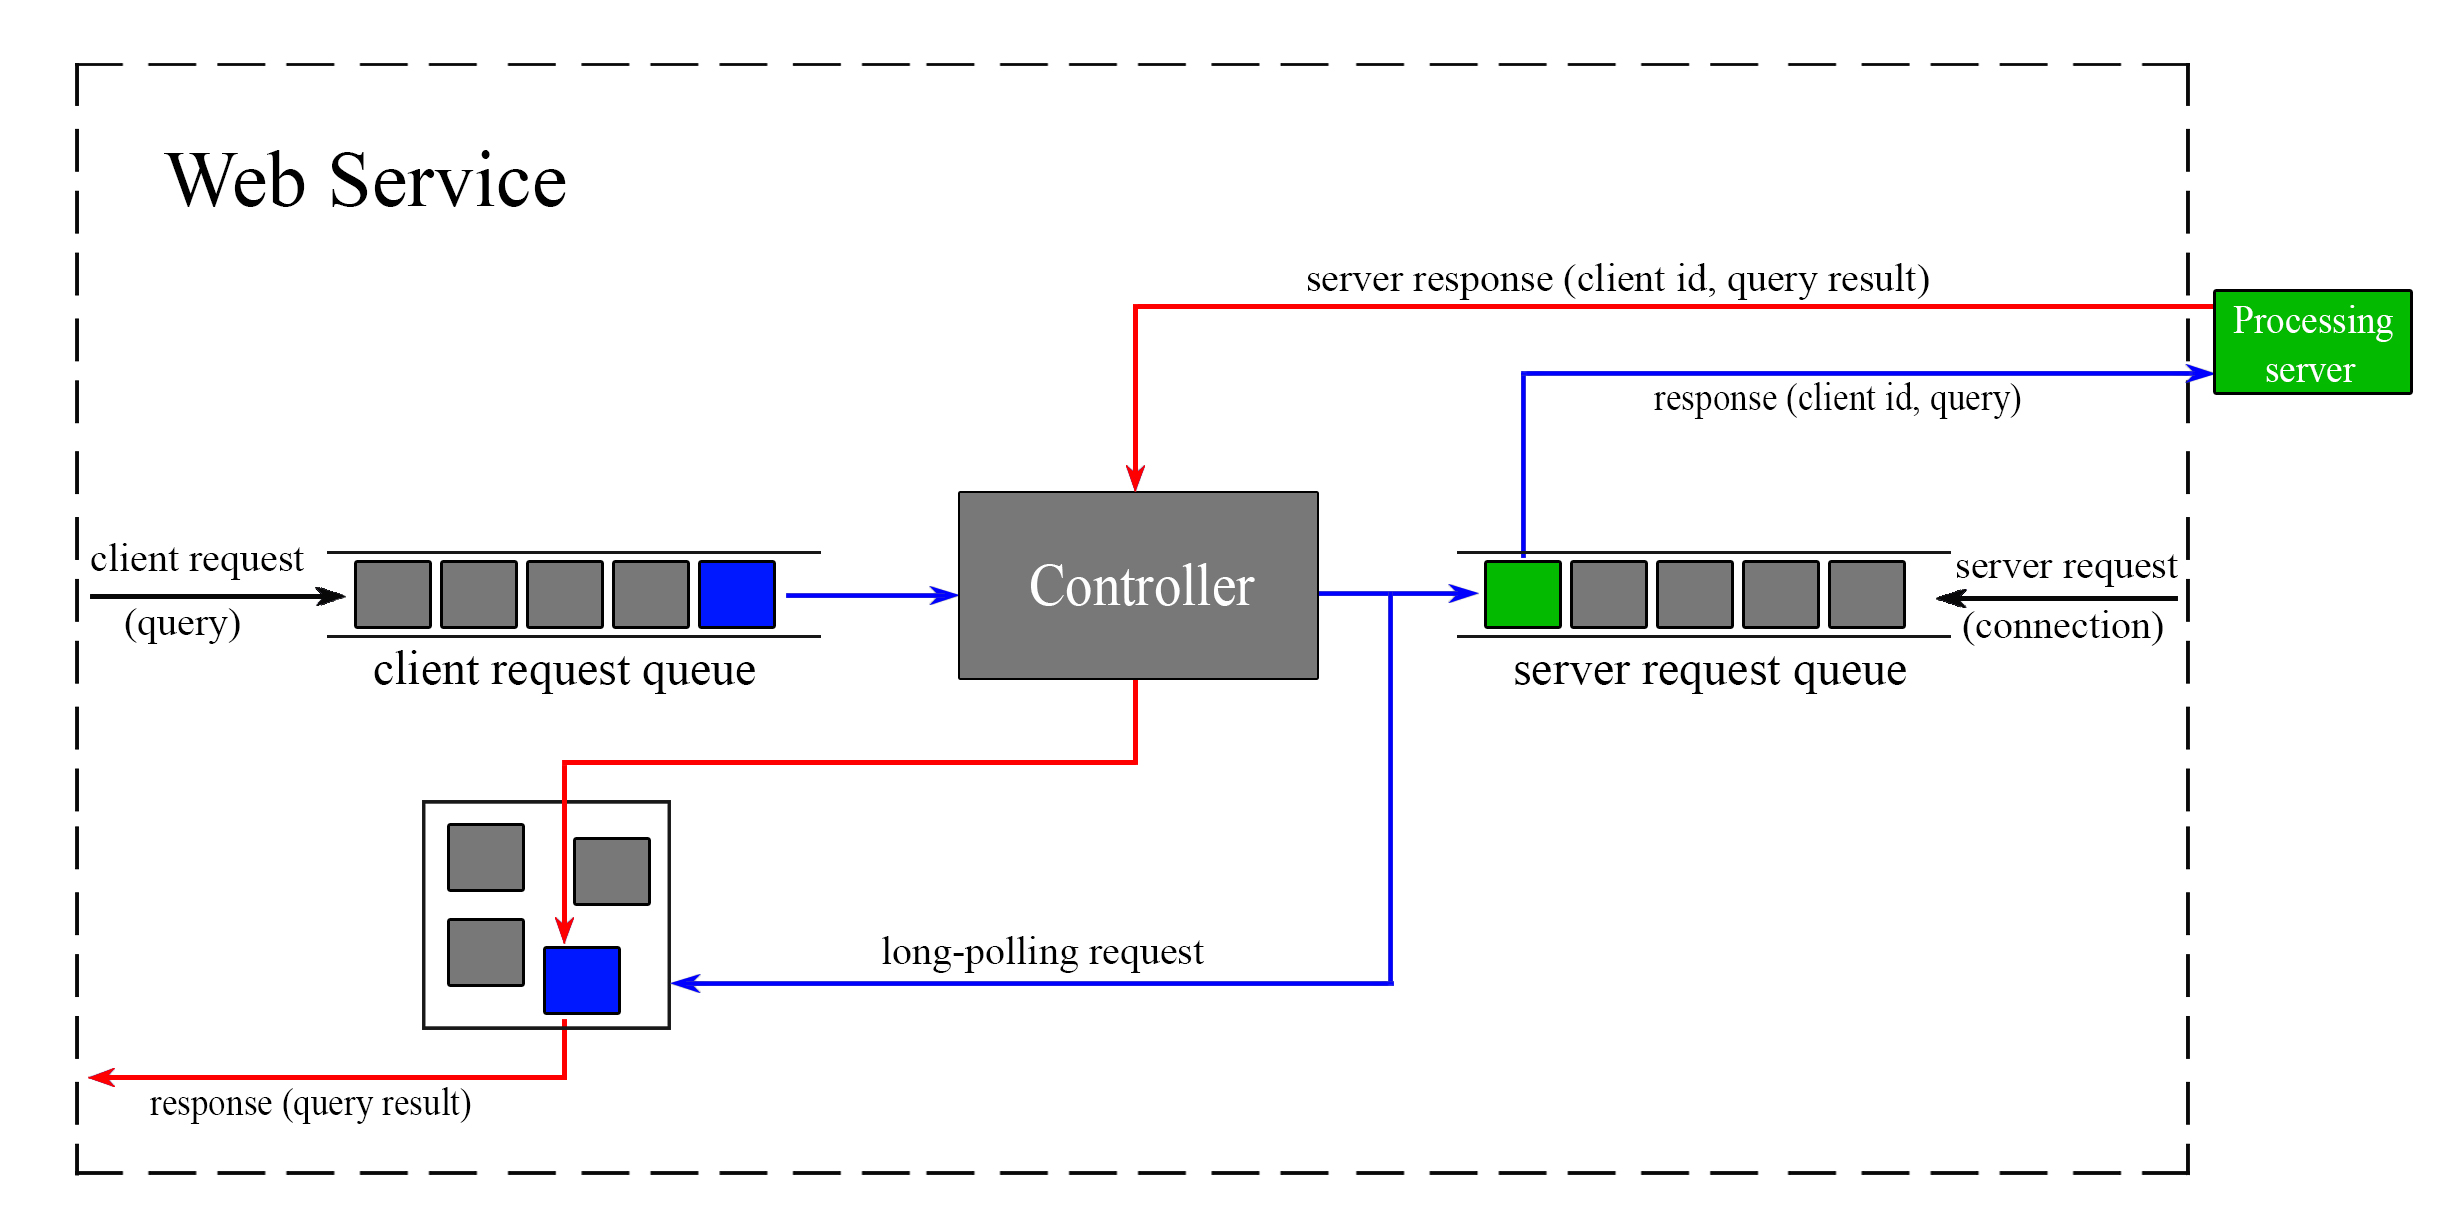
\includegraphics[scale=0.17]{ws_model}
    \else
      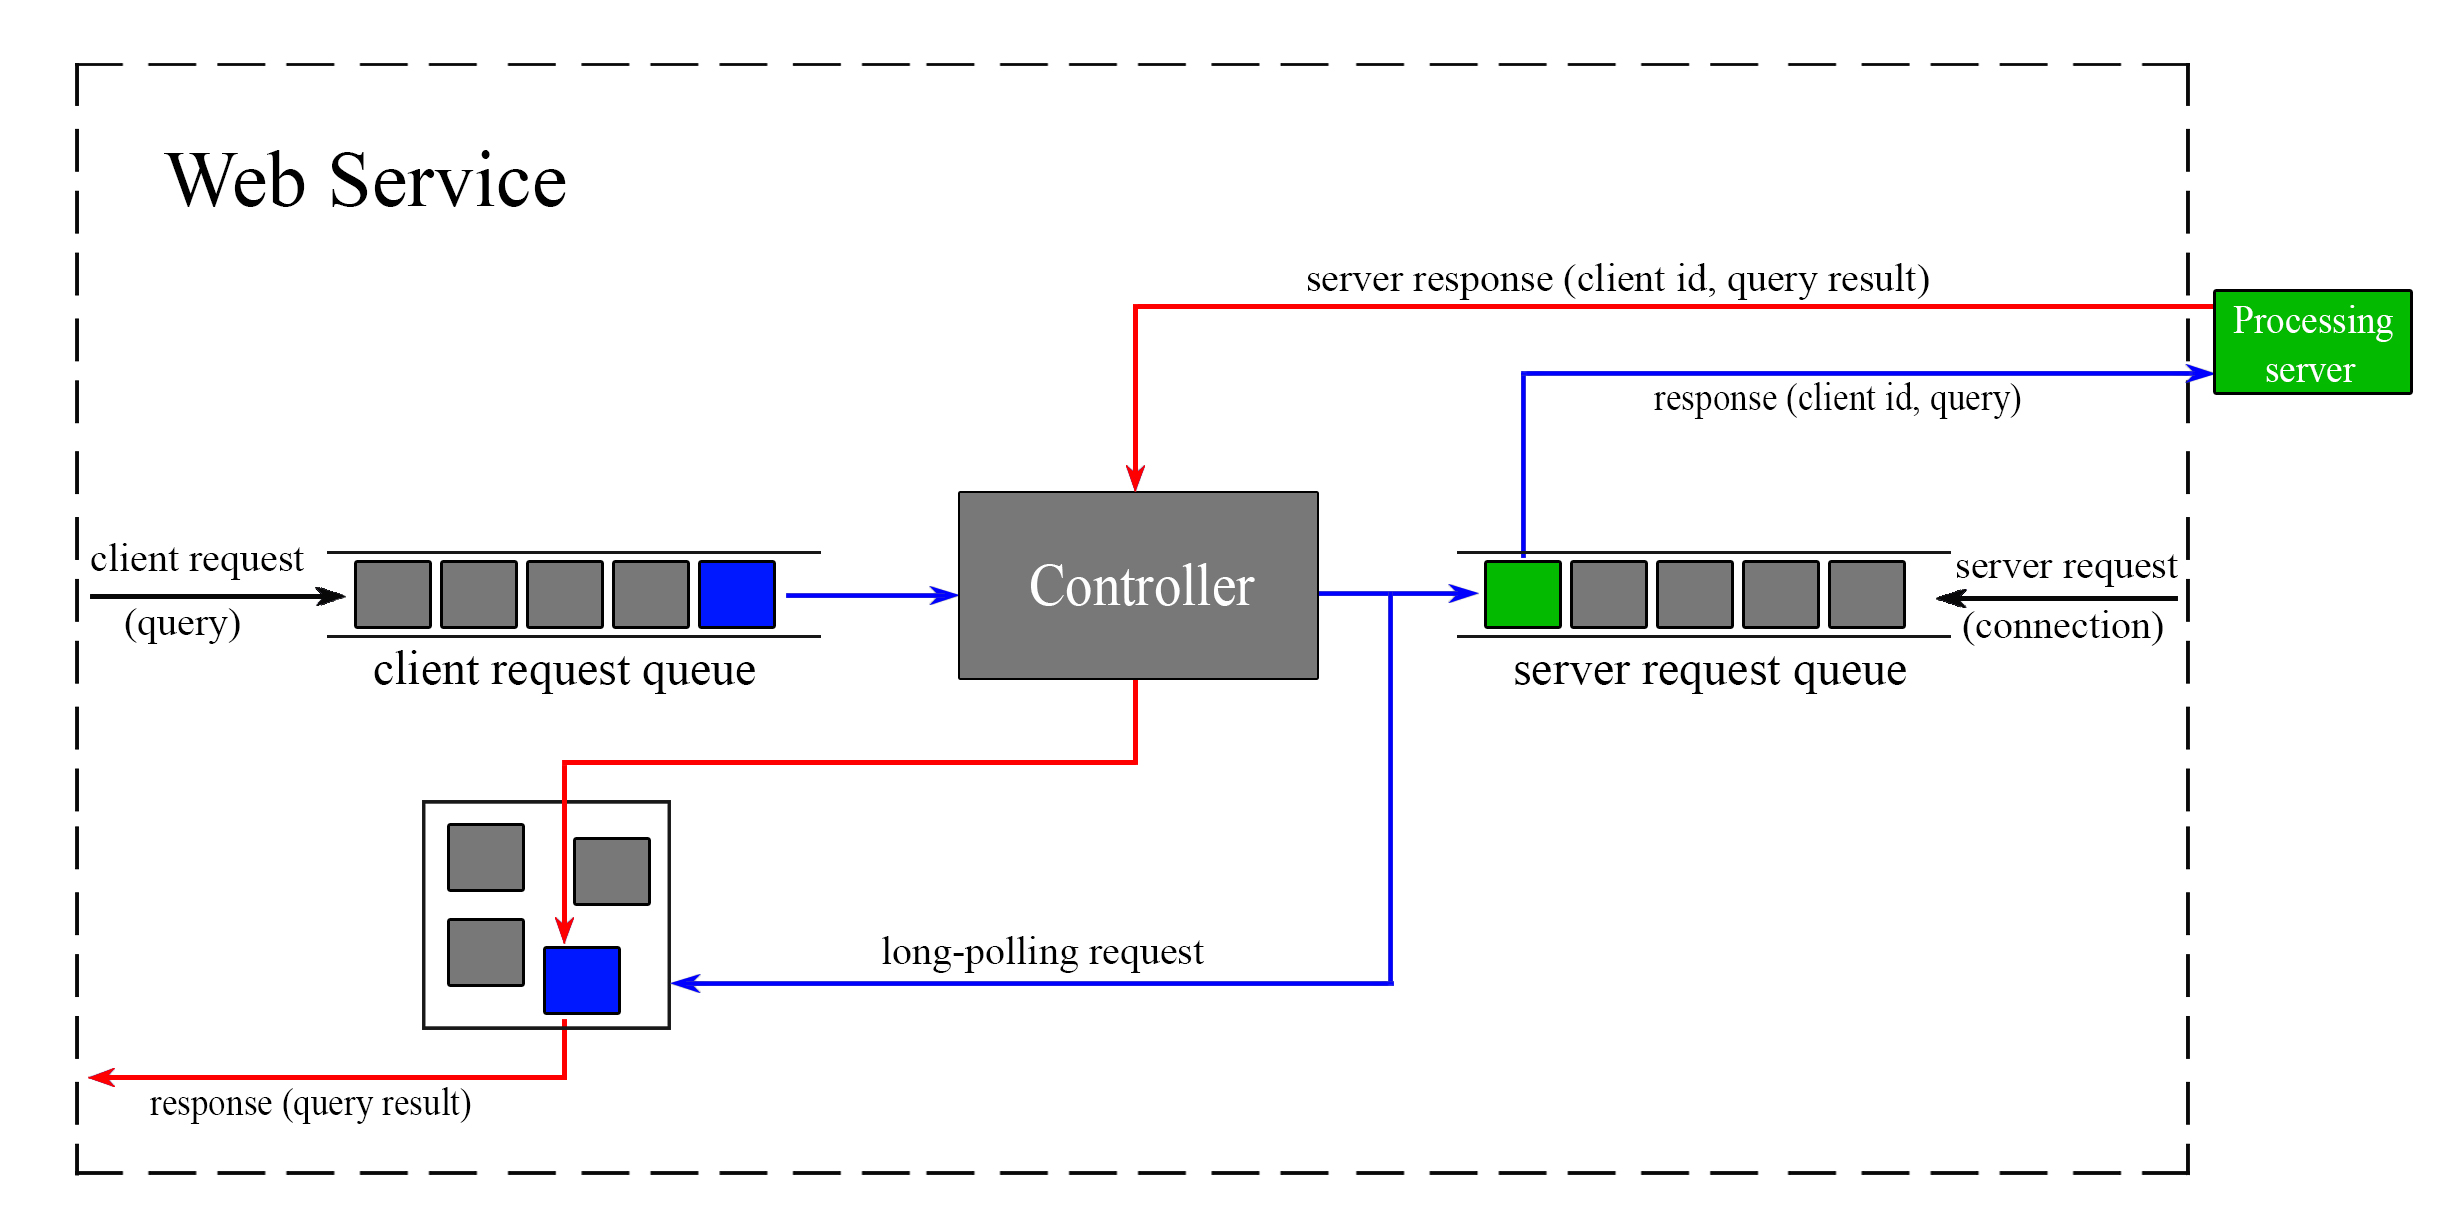
\includegraphics[scale=0.17]{ws_model}
    \fi
    \caption[Sơ đồ mô hình hoạt động chi tiết của web service]{Sơ đồ mô hình hoạt động chi tiết của web service.}
    \label{FigWS}
  \end{center}
\end{figure}


\subsubsection{Server side}
Cấu trúc của server side gồm hai thành phần chính tương ứng với hai quá trình xử lý là quá trình training và quá trình query.

Sơ đồ xử lý của quá trình training được thể hiện trong Hình \ref{FigInvertedFile}. Như đã trình bày sơ lược trong mục trong mục \ref{sec:inverted-index} và \ref{experimental-setting}, quá trình training bao gồm các bước sau:

\textbf{Dò tìm, phát hiện và rút trích đặc trưng.} Từ kho dữ liệu hình ảnh được lưu sẵn trên server, bước đầu tiên của quá trình xử lý là sử dụng phương pháp phát hiện keypoint Hessian-Affine để xác định được vị trí các điểm keypoint trên hình ảnh. Từ thông tin đó, bộ SIFT descriptor mô tả và rút trích được 1 vector 128 chiều tương ứng với mỗi điểm keypoint. Những vector này sẽ được tính RootSIFT. Các vector thu được chính là các vector đặc trưng của hình ảnh. 

\textbf{Gom cụm đặc trưng và xây dựng từ điển.} Các vector đặc trưng sẽ được gom cụm bằng thuật toán AKM để thu được các visual word với thông số k = 1 triệu. Kết quả ta sẽ thu được các visual word là các từ dùng để mô tả hình ảnh. Từ những visual word này, ta sẽ xây dựng thành một từ điển để dễ dàng cho quá trình biểu diễn và truy vấn.

\textbf{Xây dựng chỉ mục ngược.} Theo như phương pháp đề xuất đã được đề cập chi tiết trong Chương \ref{chapter:proposed}, chúng tôi sẽ xây dựng chỉ mục ngược từ từ điển nhằm đạt được hiệu suất cao trong quá trình truy vấn.

Quá trình training được thực hiện độc lập trên server và là bước tiền đề cho quá trình truy vấn.

Quá trình truy vấn được đã trình bày chi tiết trong mục \ref{sec:intergrated} và được thể hiện trong Hình \ref{FigBasicIdea}. Đầu tiên, ta sẽ rút trích đặc trưng từ hình ảnh truy vấn. Sau đó các đặc trưng này được đưa vào từ điển để lấy được các visual word tương ứng. Từ các visual word và vị trí của nó trên hình ảnh, ta sẽ dùng chỉ mục ngược áp dụng phương pháp xếp hạng voting để tìm được các ứng viên với số lượt bầu chọn nhiều nhất. Kết quả sẽ được server gửi ngược trở về webservice và trả về cho client yêu cầu.

\subsection{Giao diện}
Giao diện của ứng dụng được thiết kế đơn giản và tiện dụng với người sử dụng. Các hình ảnh screenshot của ứng dụng được thể hiện trong các hình \ref{FigChooseRegion}, \ref{FigProcessing} và \ref{FigResultCapture}.

\begin{figure}[!htbp]
  \begin{center}
    \leavevmode
    \ifpdf
      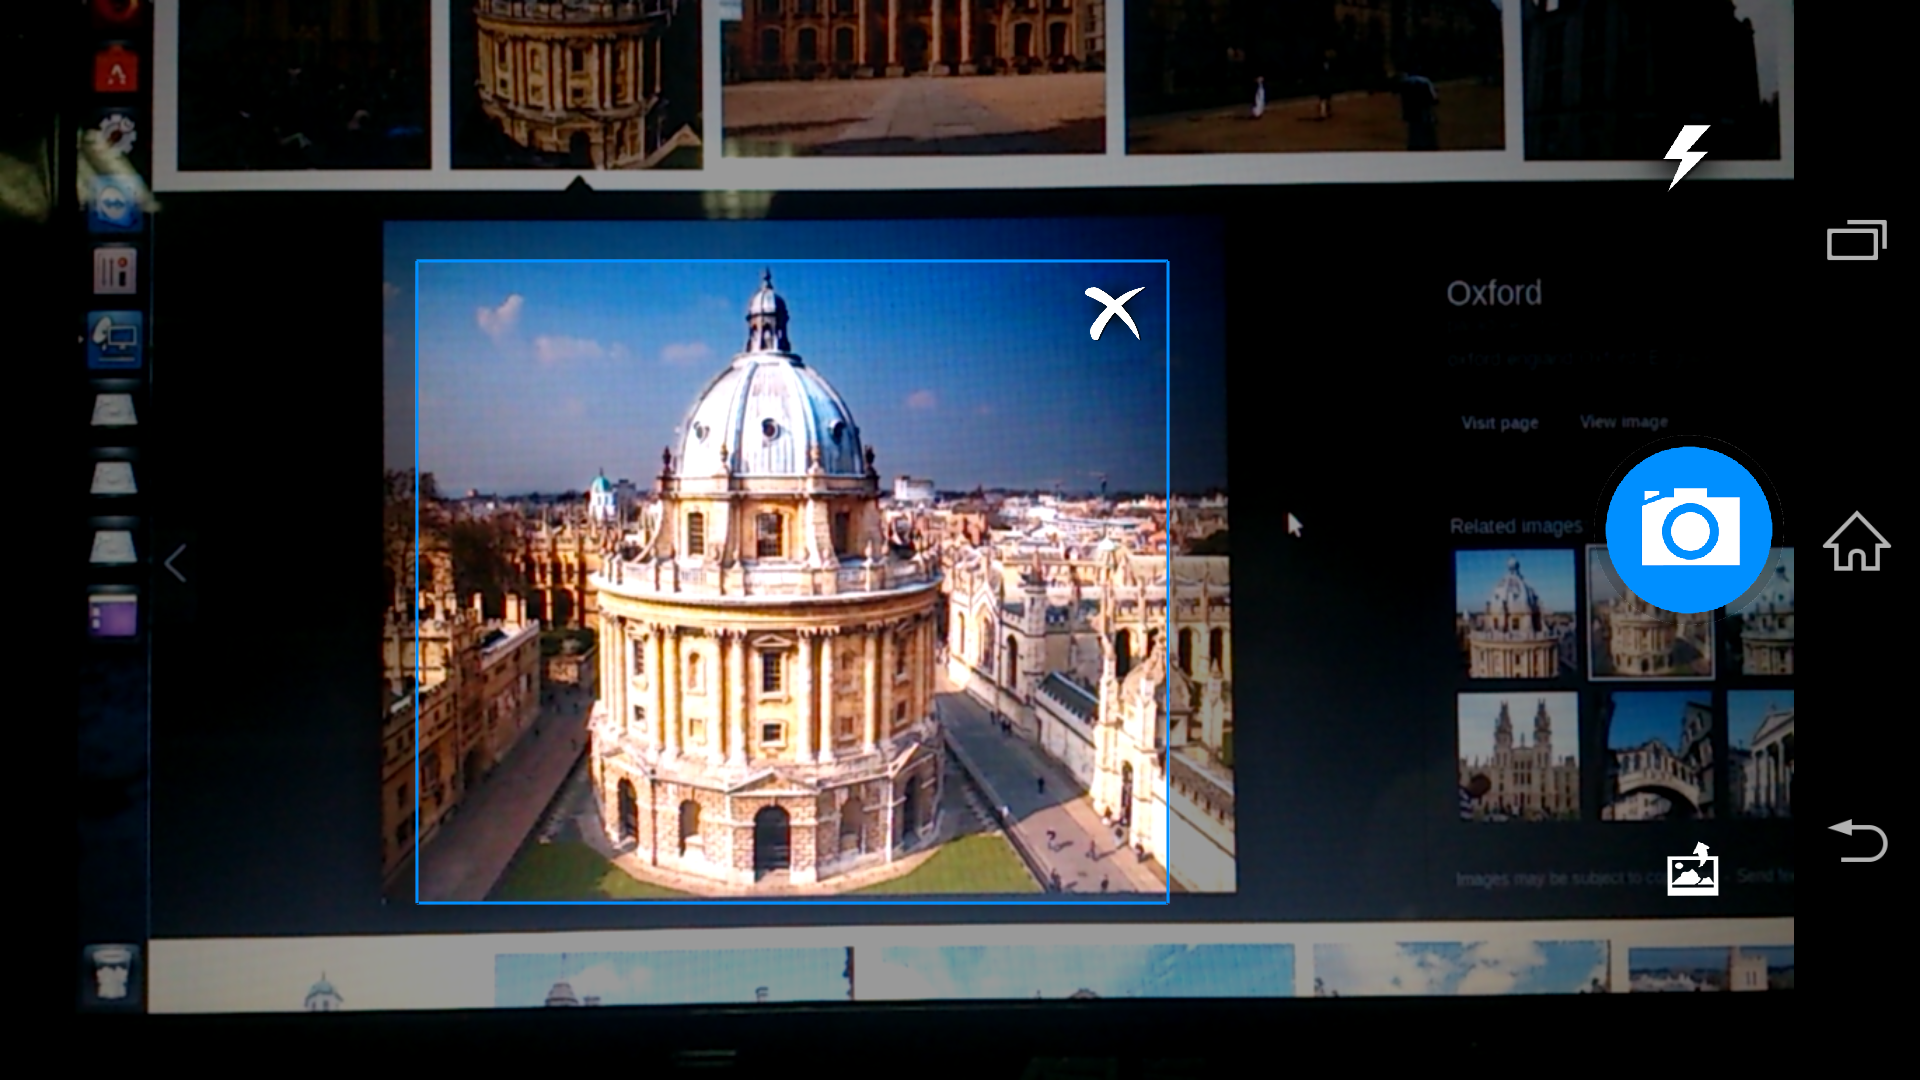
\includegraphics[scale=0.17]{choose_region}
    \else
      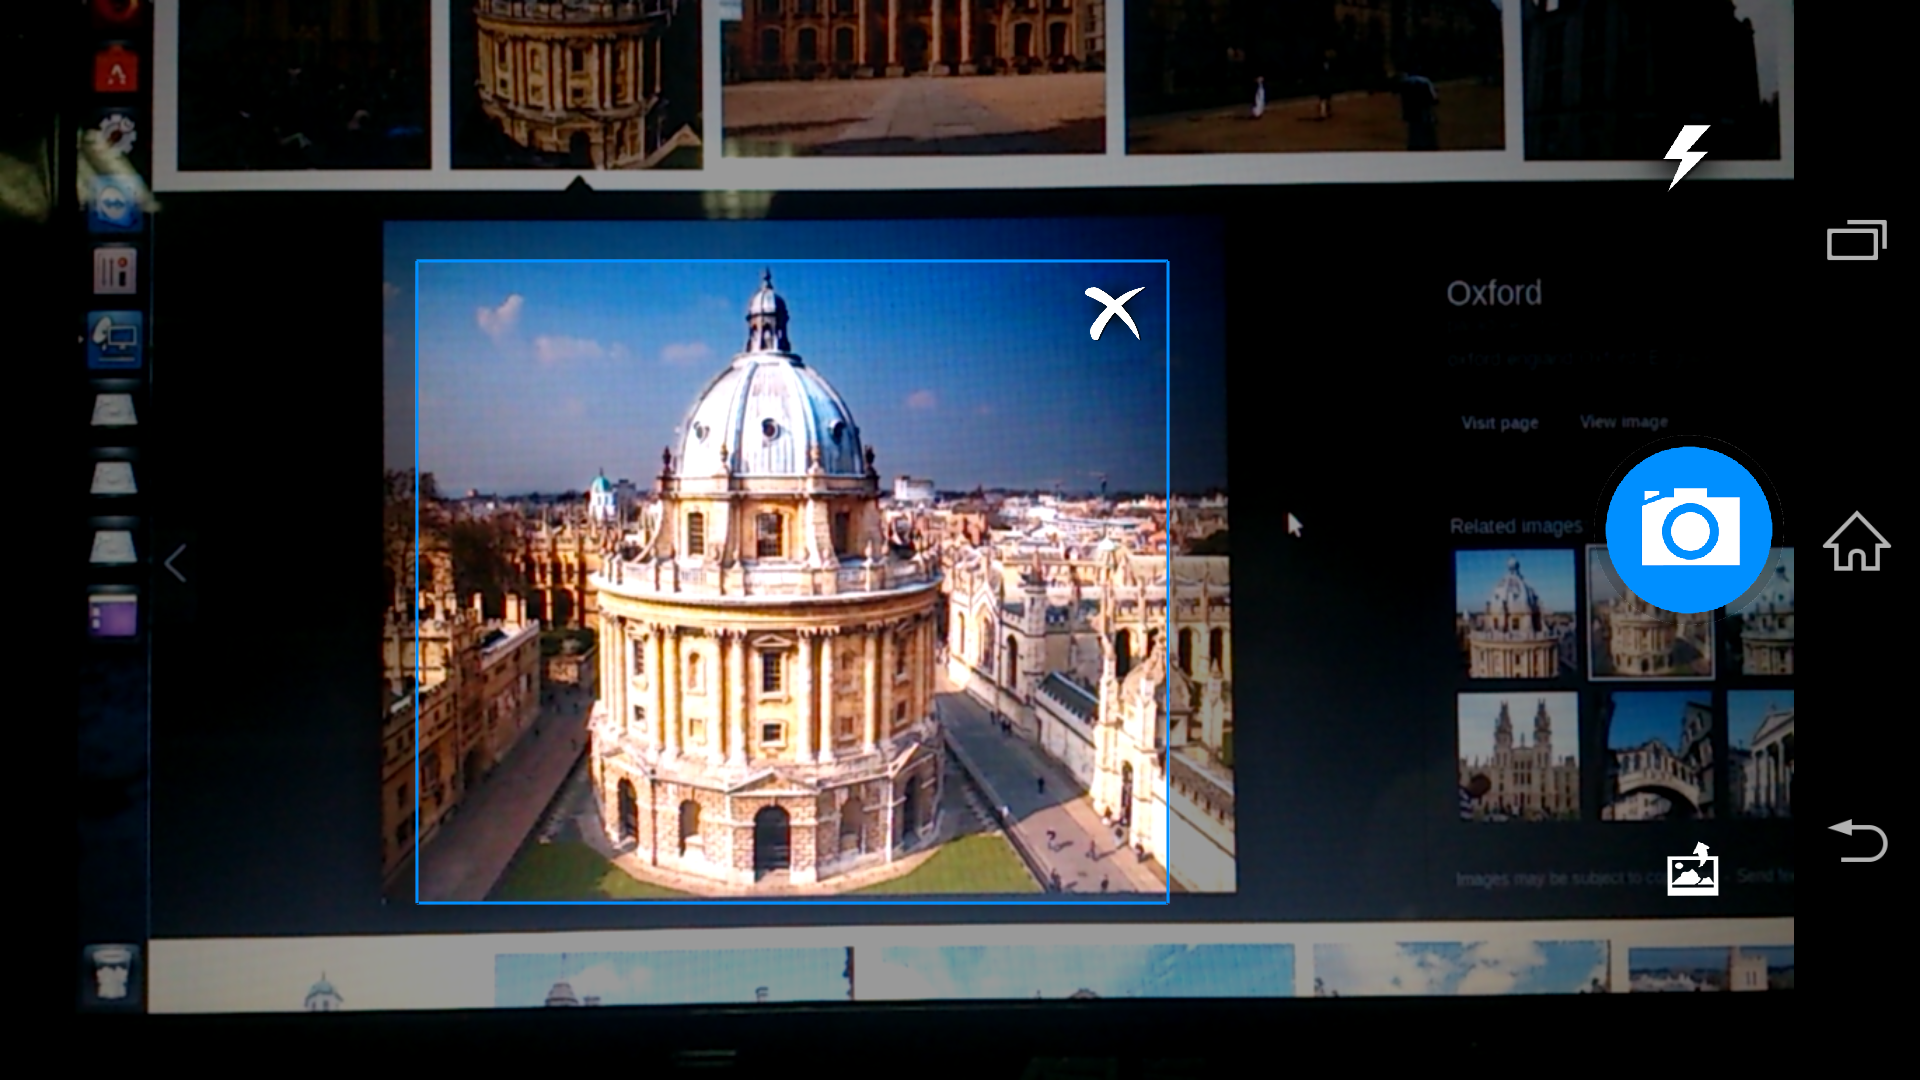
\includegraphics[scale=0.17]{choose_region}
    \fi
    \caption[Hình ảnh ứng dụng khi chọn vùng ảnh truy vấn]{Hình ảnh ứng dụng khi chọn vùng ảnh truy vấn.}
    \label{FigChooseRegion}
  \end{center}
\end{figure}

\begin{figure}[!htbp]
  \begin{center}
    \leavevmode
    \ifpdf
      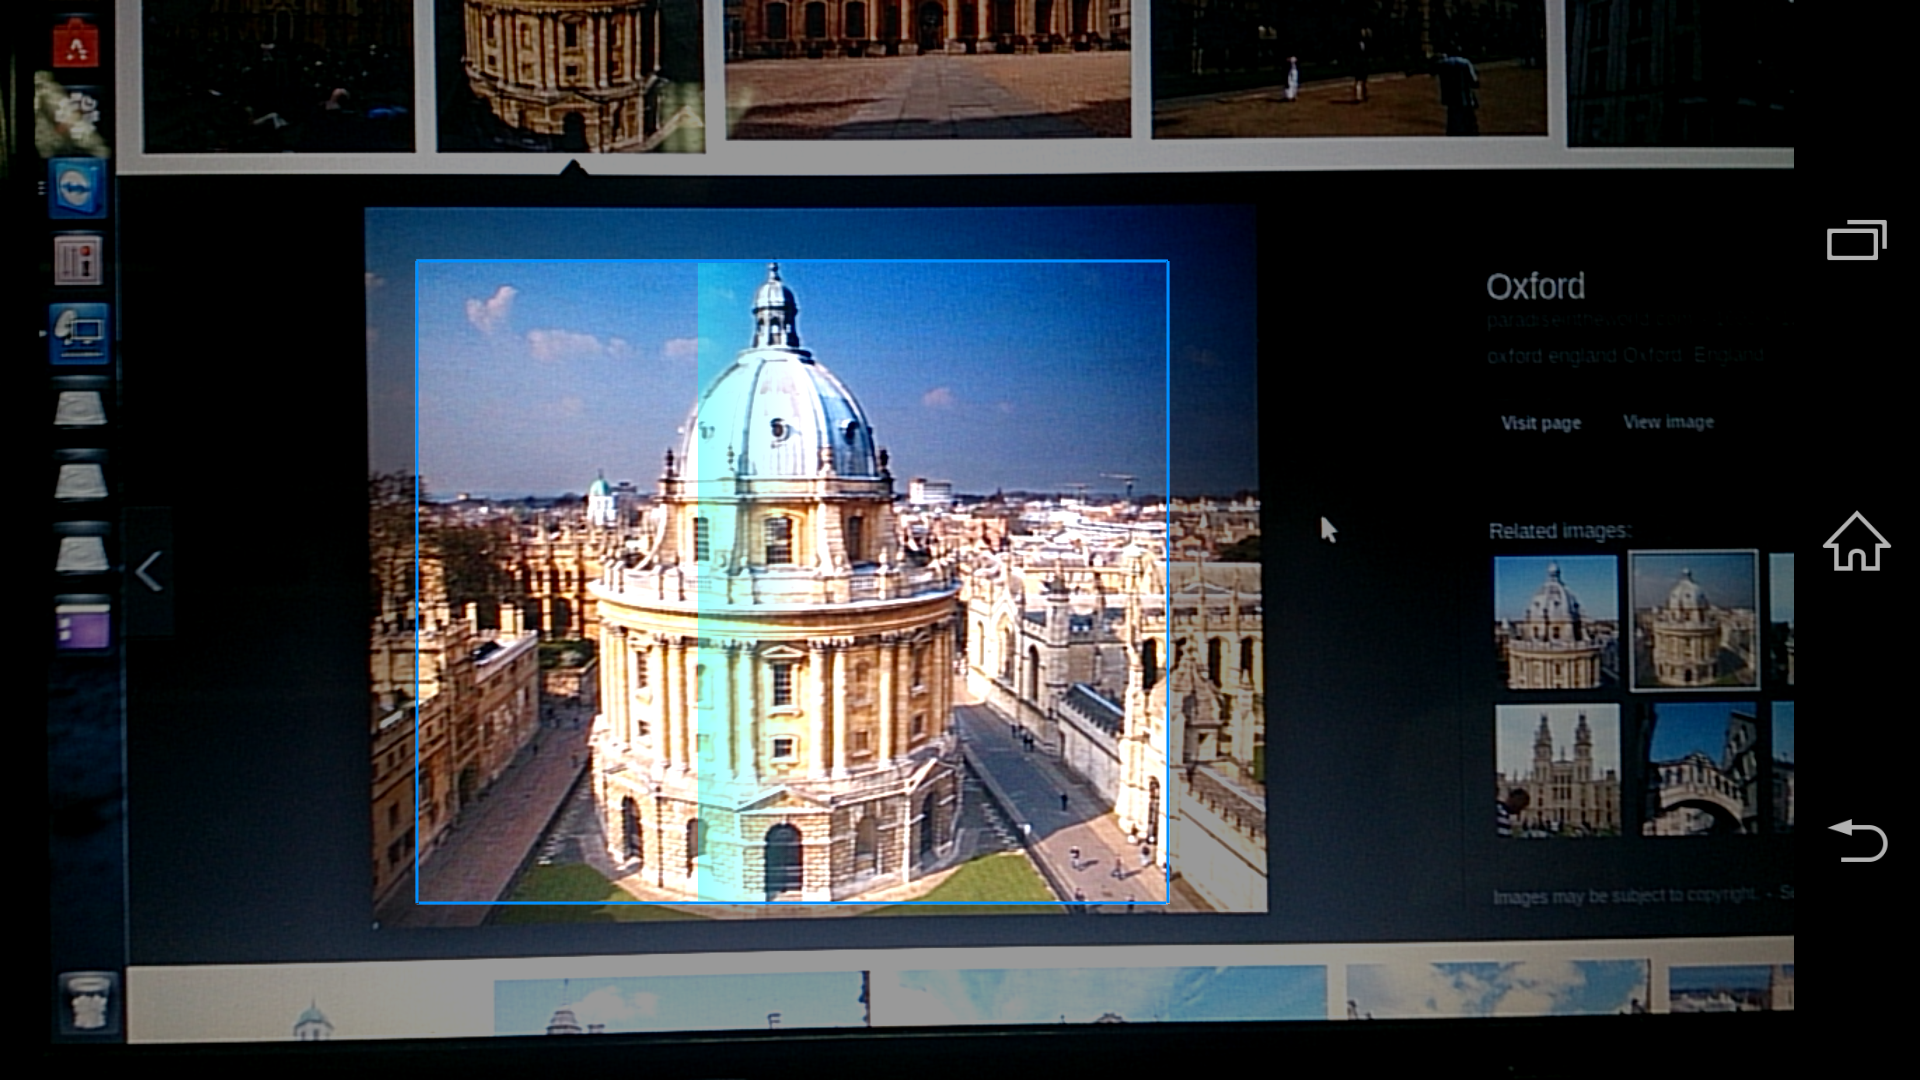
\includegraphics[scale=0.17]{processing}
    \else
      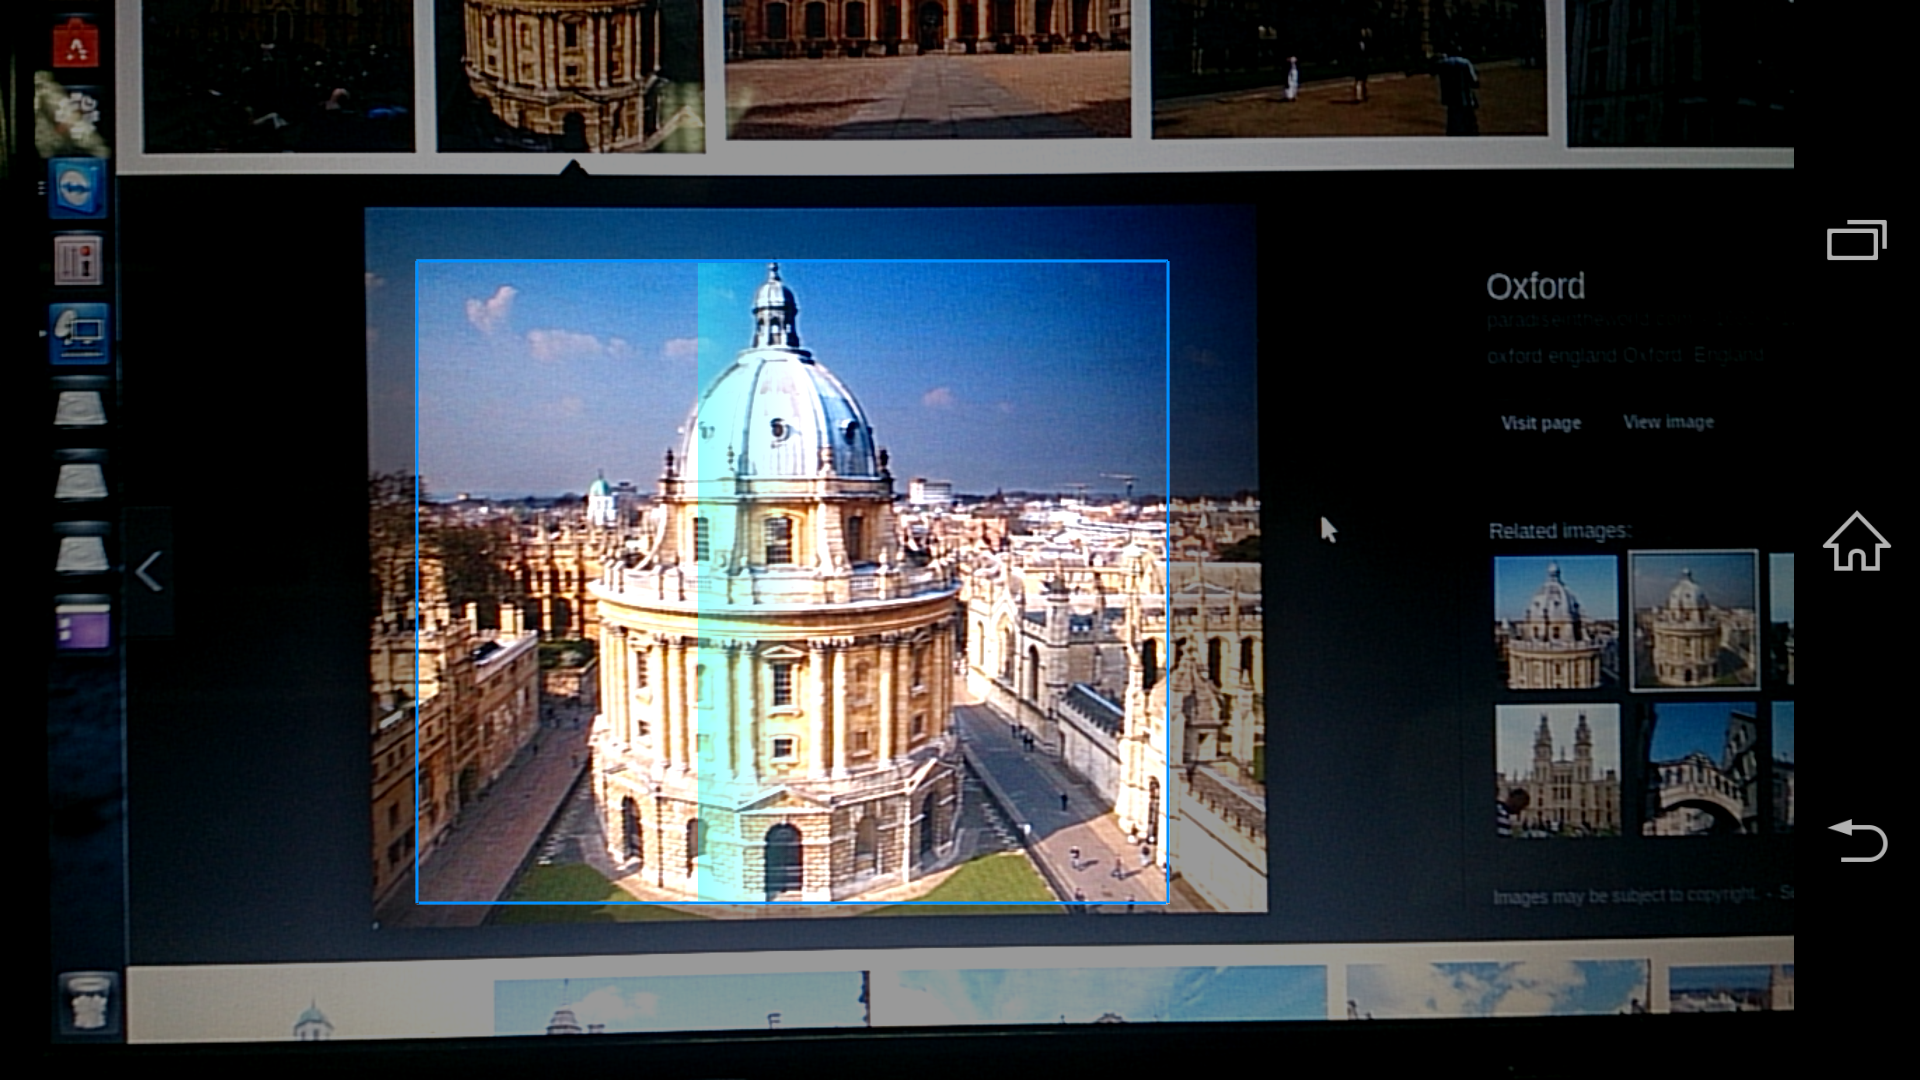
\includegraphics[scale=0.17]{processing}
    \fi
    \caption[Hình ảnh ứng dụng khi đang thực hiện truy vấn]{Hình ảnh ứng dụng khi đang thực hiện truy vấn.}
    \label{FigProcessing}
  \end{center}
\end{figure}

\begin{figure}[!htbp]
  \begin{center}
    \leavevmode
    \ifpdf
      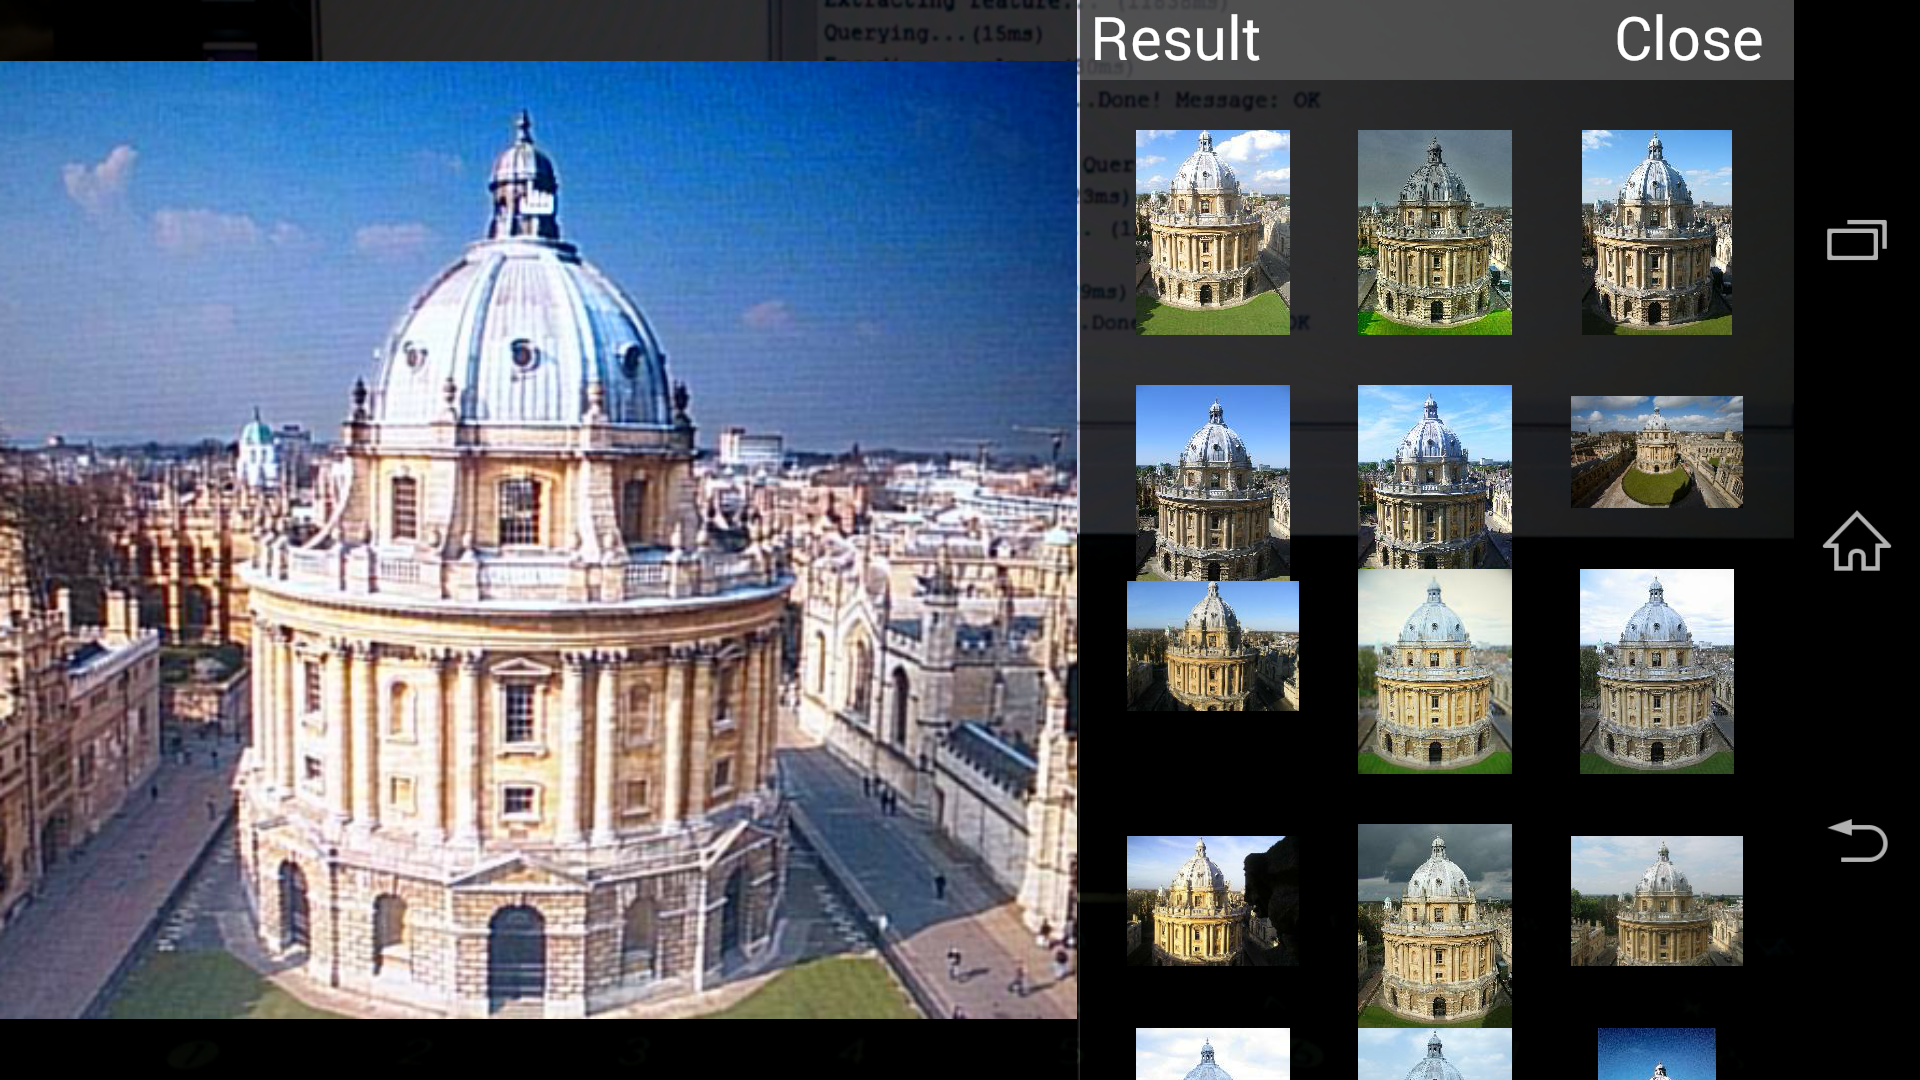
\includegraphics[scale=0.17]{result_capture}
    \else
      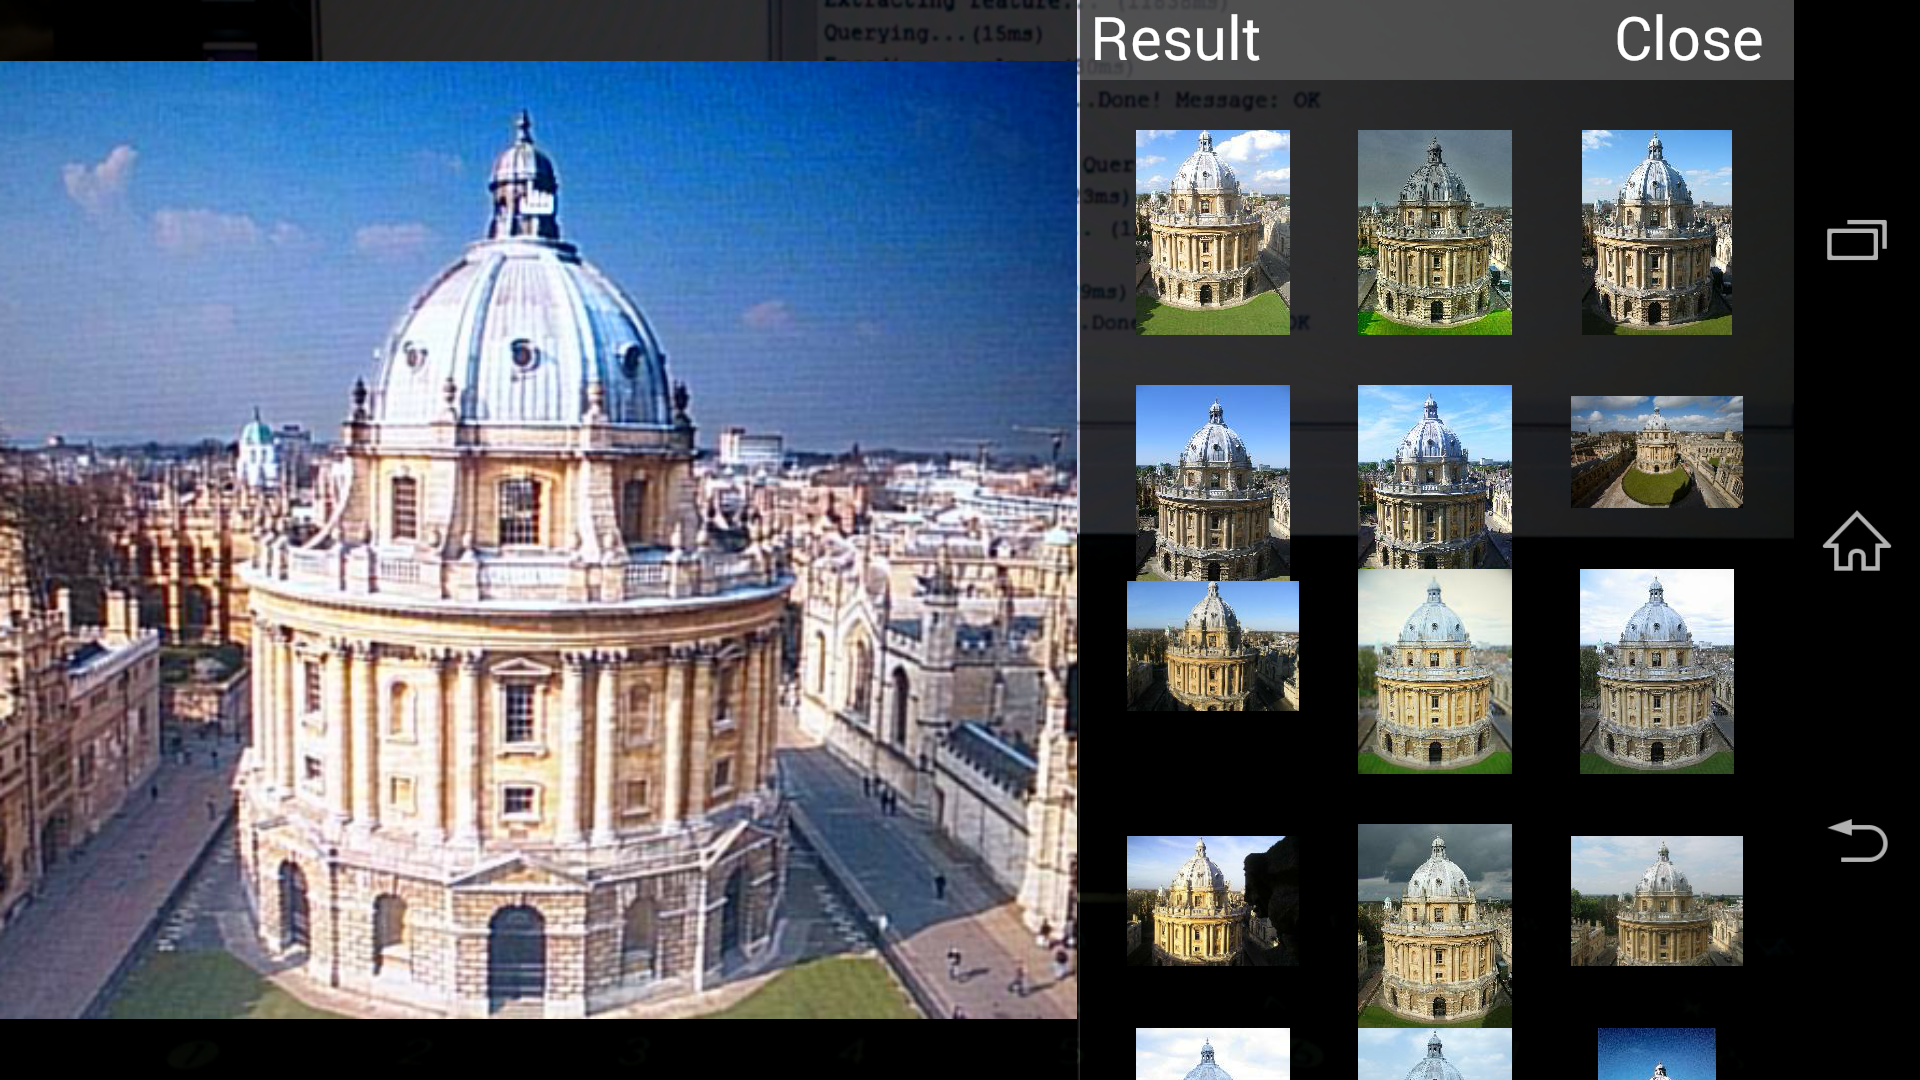
\includegraphics[scale=0.17]{result_capture}
    \fi
    \caption[Hình ảnh ứng dụng hiển thị kết quả truy vấn]{Hình ảnh ứng dụng hiển thị kết quả truy vấn.}
    \label{FigResultCapture}
  \end{center}
\end{figure}

\section{Cài đặt và thực nghiệm}
\label{c5-caidat}
	\subsection{Môi trường cài đặt}
	Môi trường cài đặt của hệ thống được liệt kê chi tiết dưới đây:
	
	\begin{itemize}
	\item \textbf{Processing Server:}
	
	-- Hệ điều hành: Windows Server 2008.
	
	-- Ngôn ngữ lập trình: Matlab, C.
	
	
	\item \textbf{Web Service:}
	
	-- Web server: Apache Tomcat 7.
	
	-- Ngôn ngữ lập trình: Java.
	
	
	\item \textbf{Client:}
	
	-- Hệ điều hành: Android.
	
	-- Ngôn ngữ lập trình: Java. 
	\end{itemize}	
	
	
	\subsection{Kết quả thực nghiệm}
	Ứng dụng nhóm xây dựng cho kết quả tốt. Ứng dụng chạy ổn định trên hệ điều hành Android. Thời gian trung bình cho mỗi truy vấn trên ứng dụng rơi vào khoảng 5 - 10s. Với những hình ảnh kích cỡ nhỏ thì thời gian truy vấn có thể chỉ trong 1s. Ngoài ra, thời gian truy vấn còn phụ thuộc vào nhiều yếu tố khác như điều kiện kết nối mạng hay chất lượng của hình ảnh truy vấn mà người dùng chọn.
	
	Ở đây, nhóm thực hiện thử nghiệm trên bộ dataset chuẩn đã dùng trong các thí nghiệm trước do đó độ chính xác không hề thay đổi so với kết quả của các thí nghiệm đã trình bày ở các chương trước.
	
	\subsection{Đánh giá kết quả}
	Kết quả thực nghiệm cho thấy ứng dụng tìm kiếm đối tượng trên ảnh đáp ứng được cơ bản các yêu cầu thực tế. Đồng thời, cách tổ chức hệ thống như trên cho phép người dùng hoàn toàn có thể scale ra nhiều server để đáp ứng được số lượng request lớn - một vấn đề mà các ứng dụng thực tế hiện nay phải đối mặt.
	
	Đồng thời, ứng dụng trên là nền tảng để phát triển vô số các ứng dụng thương mại khác vì ta có thể tùy biến trả về nhiều thông tin khác nhau tùy theo yêu cầu để ứng dụng cho nhiều lĩnh vực.